%%%---PREAMBLE---%%%%%%%%%%%%%%%%%%%%%%%%%%%%
\documentclass[oneside,12pt,final]{sty/ucthesis-CA2012}
% \pdfoutput=1

%--- Packages ---------------------------------------------------------
\usepackage[lofdepth,lotdepth,caption=false]{subfig}
\usepackage{fancyhdr}
\usepackage{hyperref}
\usepackage{amsmath, amssymb, graphicx}
\usepackage{subfig}
\usepackage{xspace}
\usepackage{braket}
\usepackage{color}
\usepackage{setspace}
\usepackage{tikz}
\usepackage{tikz-3dplot}
\tikzset{>=latex}
\usepackage{booktabs}
\usepackage[compat=1.1.0]{tikz-feynman}
%\usepackage{subfigure} (Subfigure package clashes with another package)

%---New Definitions and Commands------------------------------------------------------
\def\p{\partial}
\def\im{\mrm{im}}
\def\Tr{\mrm{Tr}}
\def\Z{\mbb{Z}}
\def\R{\mbb{R}}
\def\C{\mbb{C}}
\def\half{\frac{1}{2}}
\def\filler{\phantom{fillerfillerfiller}}
\newcommand{\be}{\begin{equation}}
\newcommand{\ee}{\end{equation}}
\newcommand{\mbb}[1]{\mathbb{#1}}
\newcommand{\mrm}[1]{\mathrm{#1}}
\newcommand{\mcal}[1]{\mathcal{#1}}
\newcommand{\mbf}[1]{\mathbf{#1}}
\newcommand{\ph}[1]{\phantom{#1}}
\newcommand{\udten}[3]{#1^{#2}_{\ph{#2}#3}}
\newcommand{\duten}[3]{#1^{\ph{#2}#3}_{#2}}
\newcommand{\pd}[2]{\frac{\p#1}{\p#2}}
\newcommand{\D}[2]{\frac{d#1}{d#2}}

%---Set Margins ------------------------------------------------------
\setlength\oddsidemargin{0.25 in} \setlength\evensidemargin{0.25 in} \setlength\textwidth{6.25 in} \setlength\textheight{8.50 in}
\setlength\footskip{0.25 in} \setlength\topmargin{0 in} \setlength\headheight{0.25 in} \setlength\headsep{0.25 in}

%%%---DOCUMENT---%%%%%%%%%%%%%%%%%%%%%%%%%%%%
\begin{document}

%=== Preliminary Pages ============================================
\begin{frontmatter}
	%%%%%%%%%%%%%%%%%%%%%%%%%%%
% TITLE PAGE INFORMATION %
%%%%%%%%%%%%%%%%%%%%%%%%%%%


\title{Simulation of MTD Performance and Measurement of Rare Higgs Decays}

\author{Jonathan Kasuke Guiang}

%%%%%%%%%%%%%%%%%%%%%%%%%%%%%%%%%%
% DECLARATIONS FOR FRONT MATTER %
%%%%%%%%%%%%%%%%%%%%%%%%%%%%%%%%%%
\report{Bachelor's Honors Thesis} \degree{Bachelor of Science} \degreemonth{June} \degreeyear{2019}
\defensemonth{May}
\defenseyear{2019}

\chair{Professor Claudio Campagnari}  % this is your advisor
\othermemberA{Professor David Stuart} % This is a member of your committee 
\othermemberB{Professor Jeffrey Richman} % This is a member of your committee 
\numberofmembers{3} % should match the number of entries above (chair + othermembers)

\field{Physics}
\campus{Santa Barbara}


%\title{{ University of California \\ Santa Barbara} \linebreak \\  Ph.D. Dissertation}
%\author{Tom\'as Andrade}
%\date{2012}

	\maketitle
	\approvalpage
	\copyrightpage
% 	\begin{dedication}

\bigskip

${}$ \\

\bigskip

${}$ \\

\bigskip

${}$ \\

\bigskip

\begin{center}
\begin{Large}
Dedication here
\end{Large}
\end{center}


\end{dedication} 
	\begin{acknowledgements}

The research included in this thesis could not have been performed if not for the assistance, patience, and support of many individuals.  I would first like to extend my deepest gratitude toward my advisor Dr. Claudio Campagnari for his mentorship and constant confidence over the course of my undergraduate studies. It was he who suggested that I study rare Higgs decays, the latter half of this thesis. He also introduced me to Dr. David Stuart, under whose advisement the former half of this thesis was performed. Claudio's support, generosity, and boundless wisdom has made me a better student and physicist.

I would additionally like to thank Dr. David Stuart. His versatile mind and constant effort to encourage learning led me to be more curious and thoughtful. Furthermore, his understanding and amiable treatment of his students promoted a positive environment for learning and practicing physics.

I would also like to extend my appreciation to Dr. Indara Suarez for believing in and guiding me - also to Nick Amin, Bennett Marsh, and Sicheng Wang for your companionship as well as helping me with anything and everything.

This research would not have been possible without the assistance of the CMS experimental collaboration who constructed the experimental apparatus and built the foundations for the data analysis.  

Finally I would like to extend my deepest thanks to my parents Orlando and Cynthia Guiang without whose love, support and understanding I could never have completed this undergraduate degree, nor would I have had the confidence or inspiration to pursue research in physics.

\end{acknowledgements} 
% 	\begin{vitae}
\addcontentsline{toc}{chapter}{Curriculum Vitae}

\begin{vitaesection}{Education}
\vspace{-0.1cm}
\item [2019]	B.S. in Physics (Expected), University of California, Santa Barbara.
\end{vitaesection}

\textbf{Publications}

Publications.

\end{vitae}
	%
%  Abstract
%

\begin{abstract}
\addcontentsline{toc}{chapter}{Abstract}
%todo: max 350 words

Progress in experimental High Energy physics can be derived from efforts in two fundamentally-linked domains: detector design and data analysis. Novel or otherwise improved detector designs push the boundaries of human perception, while rigorous, academically-motivated data analysis furthers the extent of human understanding. Therefore, both pursuits build towards the discovery of new physics, but they cannot be completely effective without the other. As such, this thesis covers them both. First, a simple, yet dynamic and effective simulation of the performance of a proposed addition to the CMS detector for the upcoming HL-LHC upgrade is described. Its programmatic construction allowed for clear and concise answers to challenging design questions posed during the upgrade's conceptual proposal and technical design. Second, a measurement of rare Higgs-boson decays, $H \rightarrow \rho+\gamma$ and $H \rightarrow \phi+ \gamma$, is performed using data based on a sample of proton-proton collisions collected by the Compact Muon Solenoid (CMS) detector at the Large Hadron Colider (LHC). Most notably, a Boosted Decision Tree (BDT) is used for distinguishing signal from background data after showing significant improvement over traditional, cut-based methods. This exploration is motivated by the possibility of measuring anomalous rates of these two particularly rare decay modes, which would reveal the existence of new physics.

%\abstractsignature
\end{abstract}



	\tableofcontents
\end{frontmatter}

\begin{mainmatter}

%---Set Headers and Footers ------------------------------------------------------
\pagestyle{fancy}
\renewcommand{\chaptermark}[1]{\markboth{{\sf #1 \hspace*{\fill} Chapter~\thechapter}}{} }
\renewcommand{\sectionmark}[1]{\markright{ {\sf Section~\thesection \hspace*{\fill} #1 }}}
\fancyhf{}

\makeatletter \if@twoside \fancyhead[LO]{\small \rightmark} \fancyhead[RE]{\small\leftmark} \else \fancyhead[LO]{\small\leftmark}
\fancyhead[RE]{\small\rightmark} \fi

\def\cleardoublepage{\clearpage\if@openright \ifodd\c@page\else
  \hbox{}
  \vspace*{\fill}
  \begin{center}
    This page intentionally left blank
  \end{center}
  \vspace{\fill}
  \thispagestyle{plain}
  \newpage
  \fi \fi}
\makeatother
\fancyfoot[c]{\textrm{\textup{\thepage}}} % page number
\fancyfoot[C]{\thepage}
\renewcommand{\headrulewidth}{0.4pt}

\fancypagestyle{plain} { \fancyhf{} \fancyfoot[C]{\thepage}
\renewcommand{\headrulewidth}{0pt}
\renewcommand{\footrulewidth}{0pt}}

%=== Introduction ============================================
\chapter{Introduction}
%
%  Introduction
%

\begin{section}{Particle Physics at the LHC}

Over the last century, the Standard Model (SM) has been shown to be the most accurate description of the fundamental construction and operation of the universe, but it is still incomplete, giving rise to many theories including Supersymmetry (SUSY), a popular extension of the Standard Model. It predicts a partner particle to every SM particle, which would resolve some particularly bothersome issues with the Standard Model like fixing the mass of the Higgs Boson, the identity of Dark Matter, and many others. Assuming SUSY is real, supersymmetric particles are expected to appear in high-energy collisions at the Large Hadron Collider (LHC). However, direct evidence for SUSY, or for any other competing theory, has yet to be discovered. Therefore, the pursuit of direct discoveries of new physics -- where ``new physics" is herearfter used to refer to evidence for Beyond Standard Model (BSM) particles -- is in a state of flux at the time of writing, and there is a growing doubt within the High Energy community that any discovery is likely to be made in the near future (i.e. within the next century). In response, CERN is investing in enhancing the LHC itself, first during a brief, two-year (2019 to 2021) shutdown period, then during a much longer overhaul for the High-Luminosity LHC (HL-LHC) with the hope that upgraded software and hardware and an enormous increase in data from the HL-LHC will push the field forward. In addition, contributions from the LHC may come from an analysis philosophy that does not fit the popular conception of scientific progress: rather than focusing on finding direct evidence of new physics, perhaps it is more useful to find new inconsistencies with the Standard Model to point future experiments in the right direction. This philosophy has always existed, and many such studies have been performed, but it has had understandably little recognition compared to achievements like the famous discovery of the Higgs boson. However, raising new, concerning questions is just as important as discovering their answers, since the former motivates the latter. In the context of experiments at the LHC, raising a concerning question is as simple as poking another hole in the Standard Model, but the question is only useful if it is more answerable than questions like a seventy-percent deficit in the current description of the makeup of the universe (dark matter) or the possibility of the quantization of gravity at energy scales beyond comprehension (gravitons). Nevertheless, there is a future worth watching at the LHC.

\end{section}

\begin{section}{The Compact Muon Solenoid}

The Compact Muon Solenoid (CMS) is a general purpose detector at the LHC, meaning it probes for the existence of a variety of new physics. The detector's namesake is a ``compact'' solenoid, the largest superconducting magnet ever built (with a length of 15m and diameter of 7m), that generates a 4T magnetic field strong enough to pull many high-energy, charged particles produced in a proton-proton collision towards CMS's detector layers\cite{CMS:1994hea}. Particles first encounter the tracker, which is composed of several layers of silicon pixels and strip detectors. Essentially, a through-going particle leaves a cascading charge deposit that can be measured as an electrical signal. This results in an accurate measurement of the particle's position as it passes through various sections of the tracker, which can then be reconstructed to give the particle's entire trajectory. Track information provides fundamental insights like the charge and momentum of a particle, for instance, which can be inferred from the curvature of the particle's trajectory. Having passed through the tracker, particles then encounter the calorimeters, which will measure the final energies of emergent particles when possible. Energies of particles that interact by the electromagnetic force, electrons and photons, are measured by the Electromagnetic Calorimeter (ECAL) while those that interact by the strong force, hadrons, are measured by the Hadronic Calorimeter (HCAL). Finally, particles that escape the ECAL and HCAL -- now only muons and weakly interacting particles -- encounter the muon layer, where muons are tracked further, before leaving the bounds of CMS. The presence of neutrinos, which mostly pass through the detector undisturbed, and possibly yet-undiscovered particles can only be inferred. Conservation of momentum is key here: invisible particles will show up as missing energy in comparing the sum of the measured particle momenta to the overall energy of the collision.

\begin{figure}[htb]
\begin{center}
\subfloat[Cutaway view of CMS detector.]      {
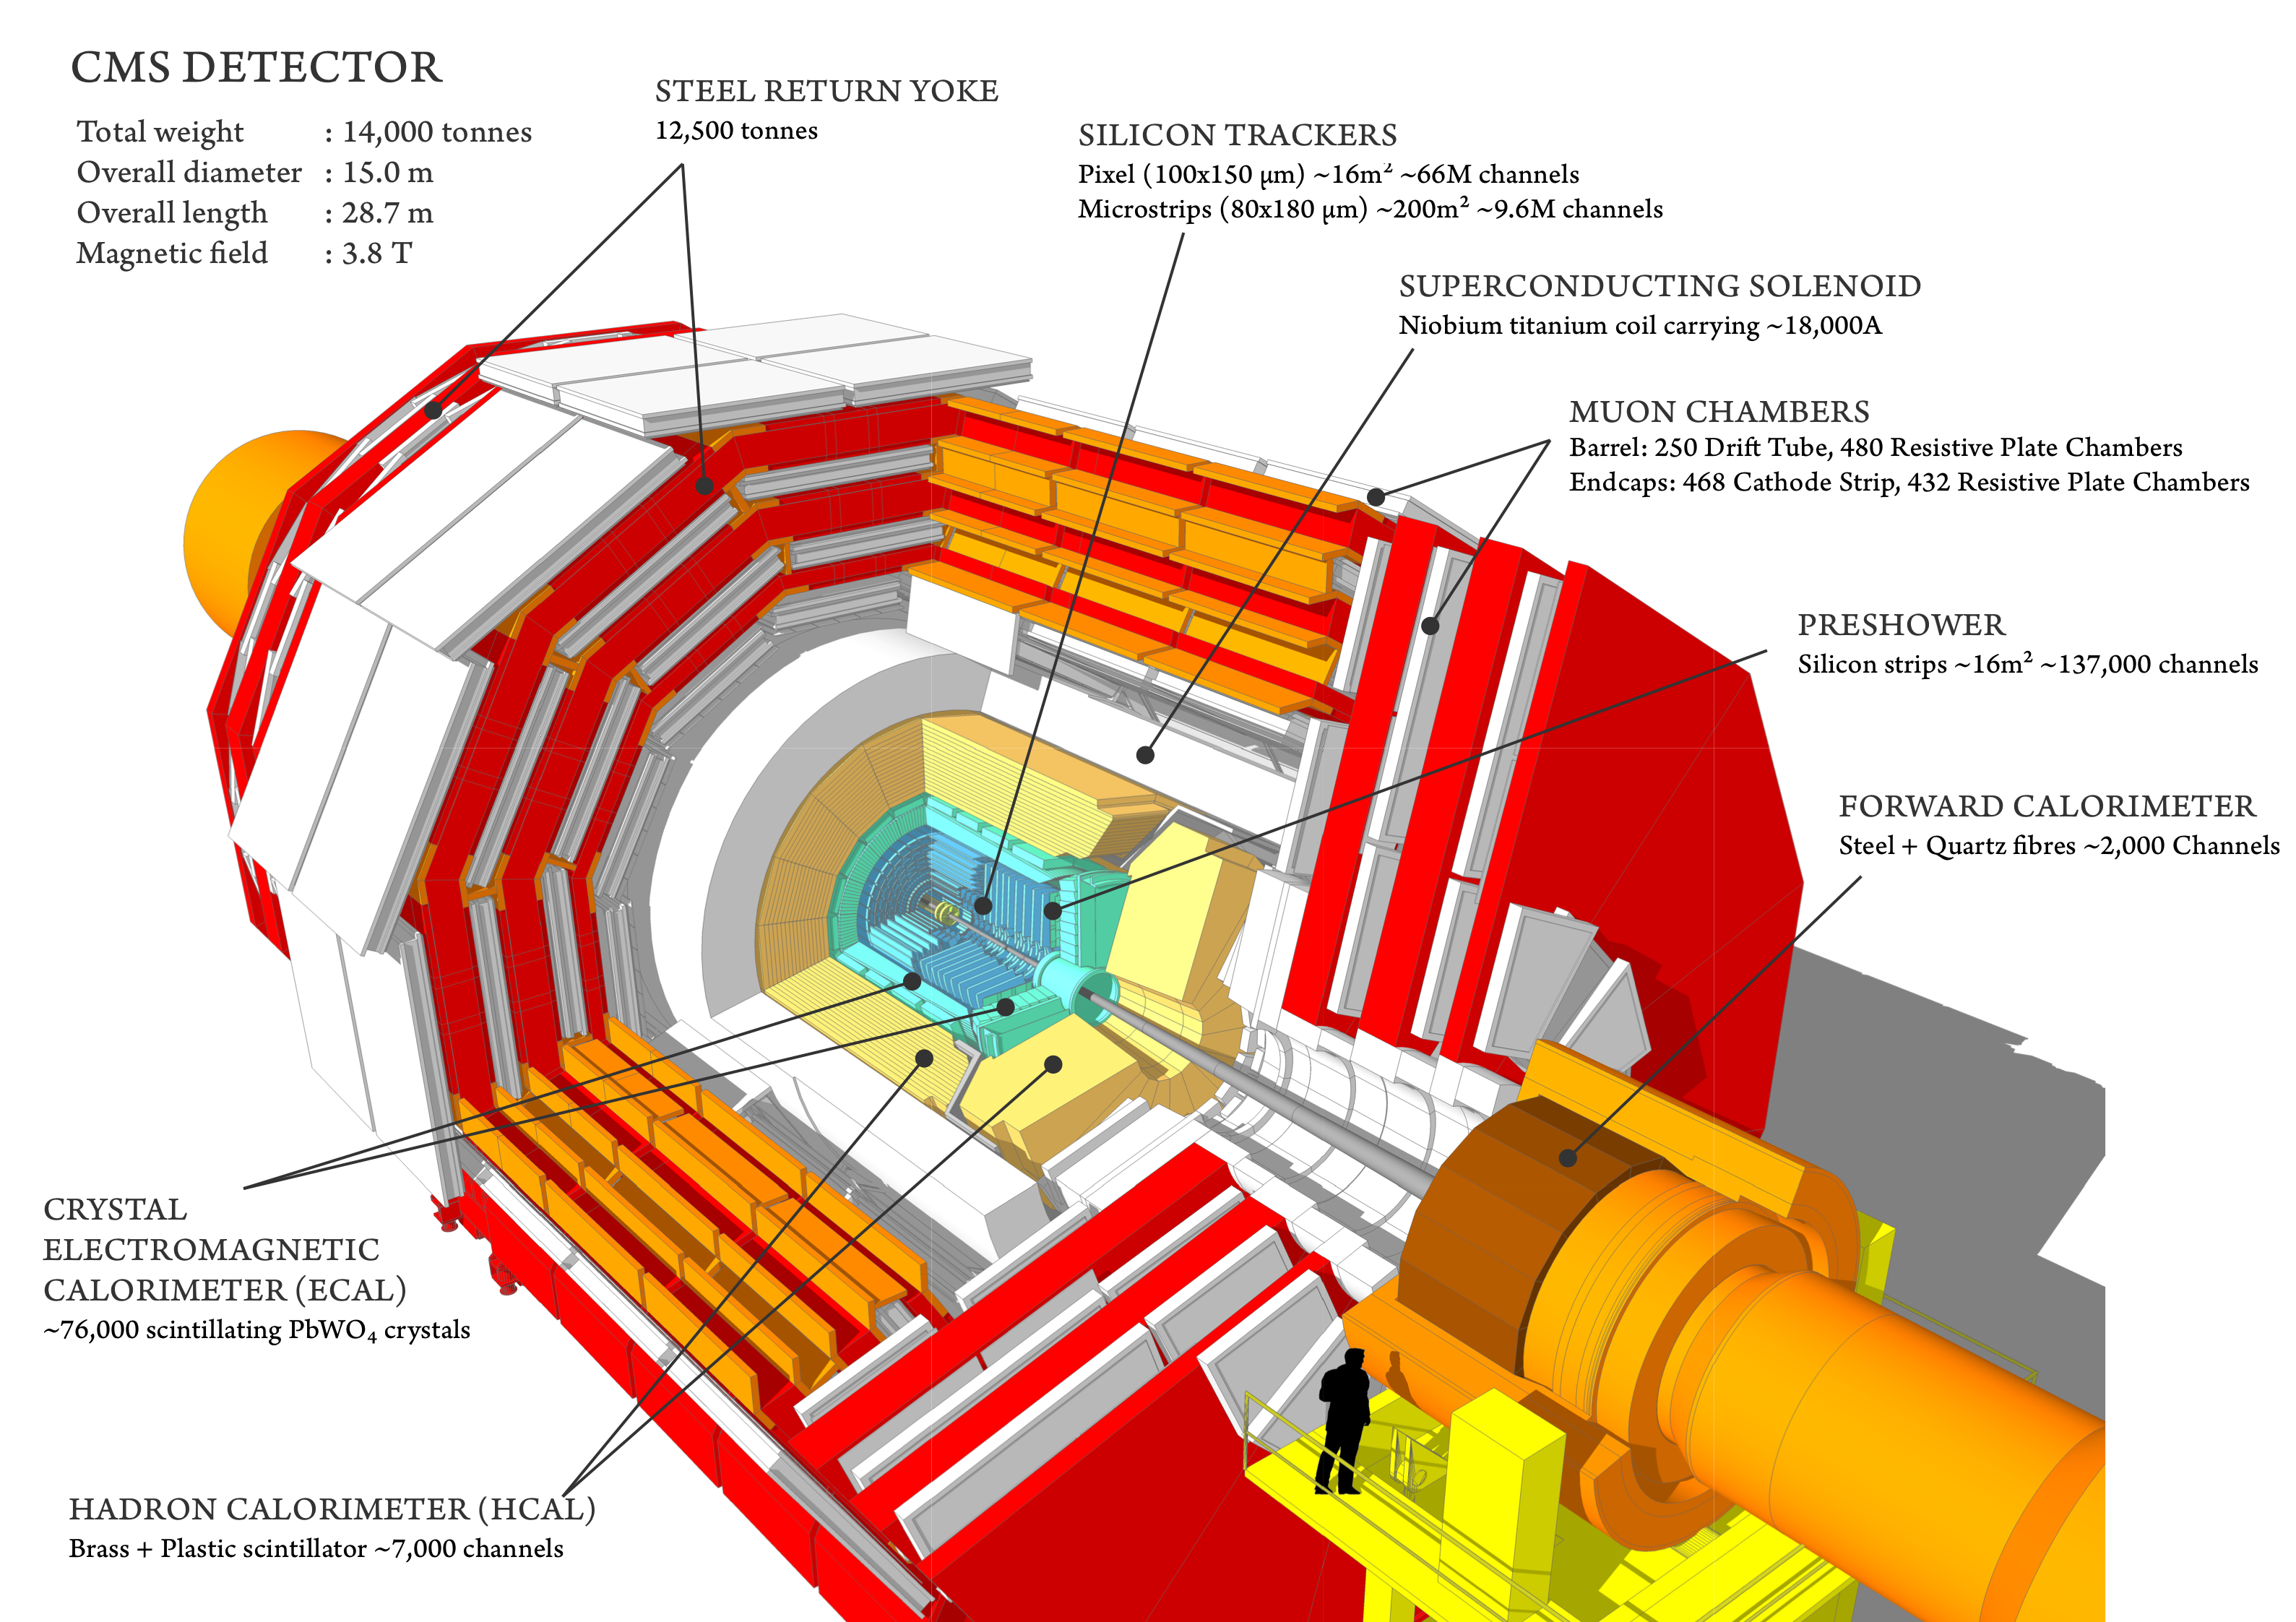
\includegraphics[width=.45\linewidth]{Dissertation/fig/cms-xsec.png}
}\quad
\subfloat[Illustration of detector layer response.]      {
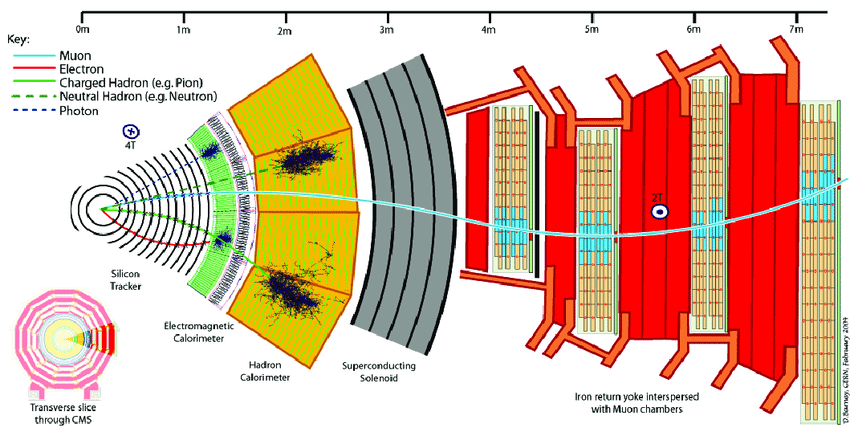
\includegraphics[width=.45\linewidth]{Dissertation/fig/cms-slice.png}
}
\end{center}
\caption{Visualizations of the design and function of CMS.}
\label{fig:cms-xsec}
\end{figure}

\end{section}

%=== Chapter 2  ============================================
\chapter{MTD Simulation}
%
%  MTD Simulation
%

\begin{section}{Motivation}

The HL-LHC upgrade will offer unprecedented luminosity in which one may find new physics, but it brings with it new complications that must be addressed by upgraded or additional detector hardware. Foremost among the new challenges posed by the HL-LHC is that higher luminosity means many more particles, which provides a far more complex picture to reconstruct for analysis. One such complexity is the increase in collision points, which is a key component of both offline and online reconstruction. With more particles colliding, collision points start to ``pile up'' on top of each other in space (this phenomena is aptly referred to as \textit{pileup}). Consequently, when reconstructing collisions into discrete ``events,'' one for each proton-proton collision, the reconstruction algorithm is unable to discern between one collision and many others that occurred in the same point in space. However, these collisions occur at different \textit{times}, so adding timing information should certainly help reduce pileup. In fact, this has been studied and proven to be the case in simulations (Fig. \ref{fig:pileup-reduce}). To this end, it has been proposed that a layer of silicon-based sensors called the MIP Timing Detector (MTD), with sufficient timing resolutions, be placed around the perimeter -- surrounding the barrel and covering the endcap -- of the CMS detector, but the design and approval of such an upgrade is no simple task. From its conceptual inception to the finalization of its technical design, questions continually arise, so clear, cogent answers are constantly required, but since the detector has yet to be built, computer simulations are necessary to address these important concerns regarding the design and projected performance of the MTD.

\begin{figure}[htb]
\begin{center}
\subfloat      {
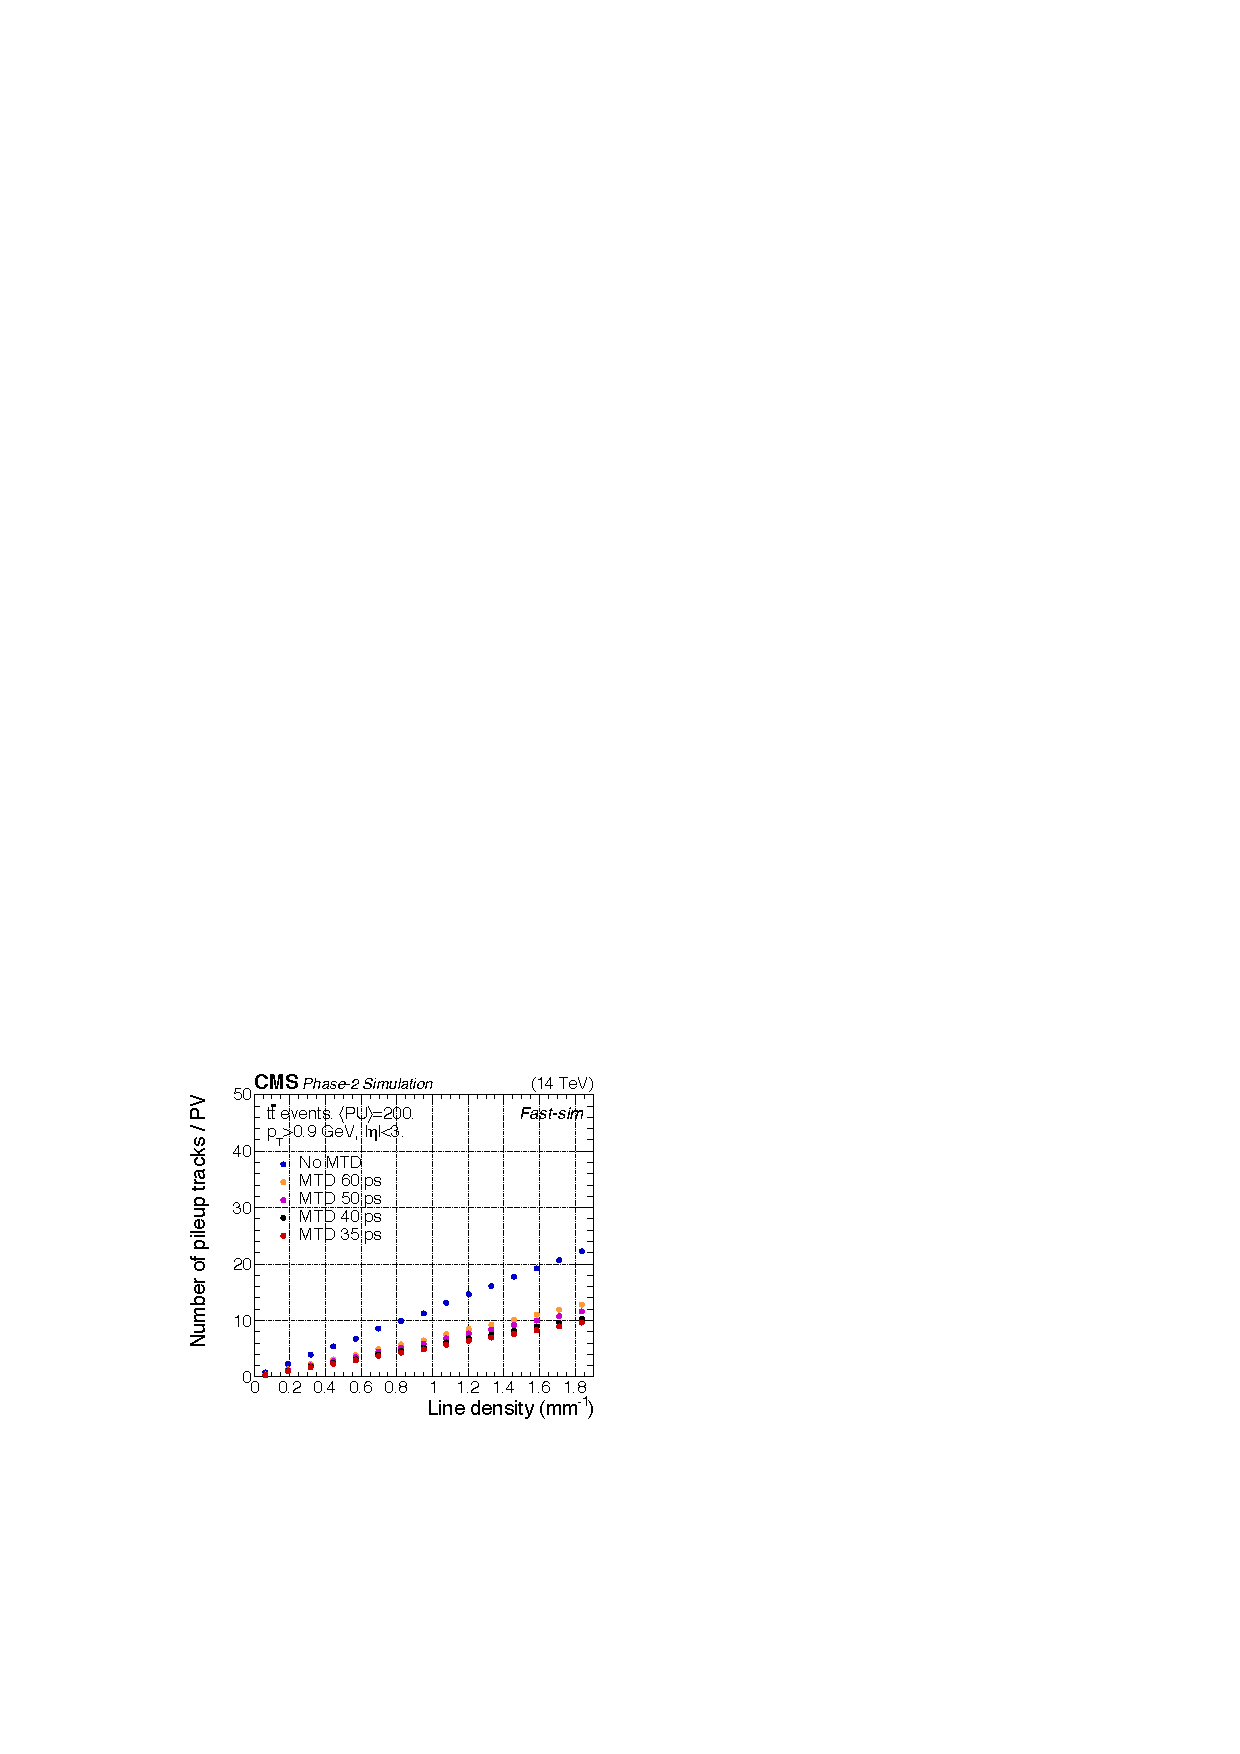
\includegraphics[width=.45\linewidth]{Dissertation/fig/pileup-reduce1.pdf}
}\quad
\subfloat      {
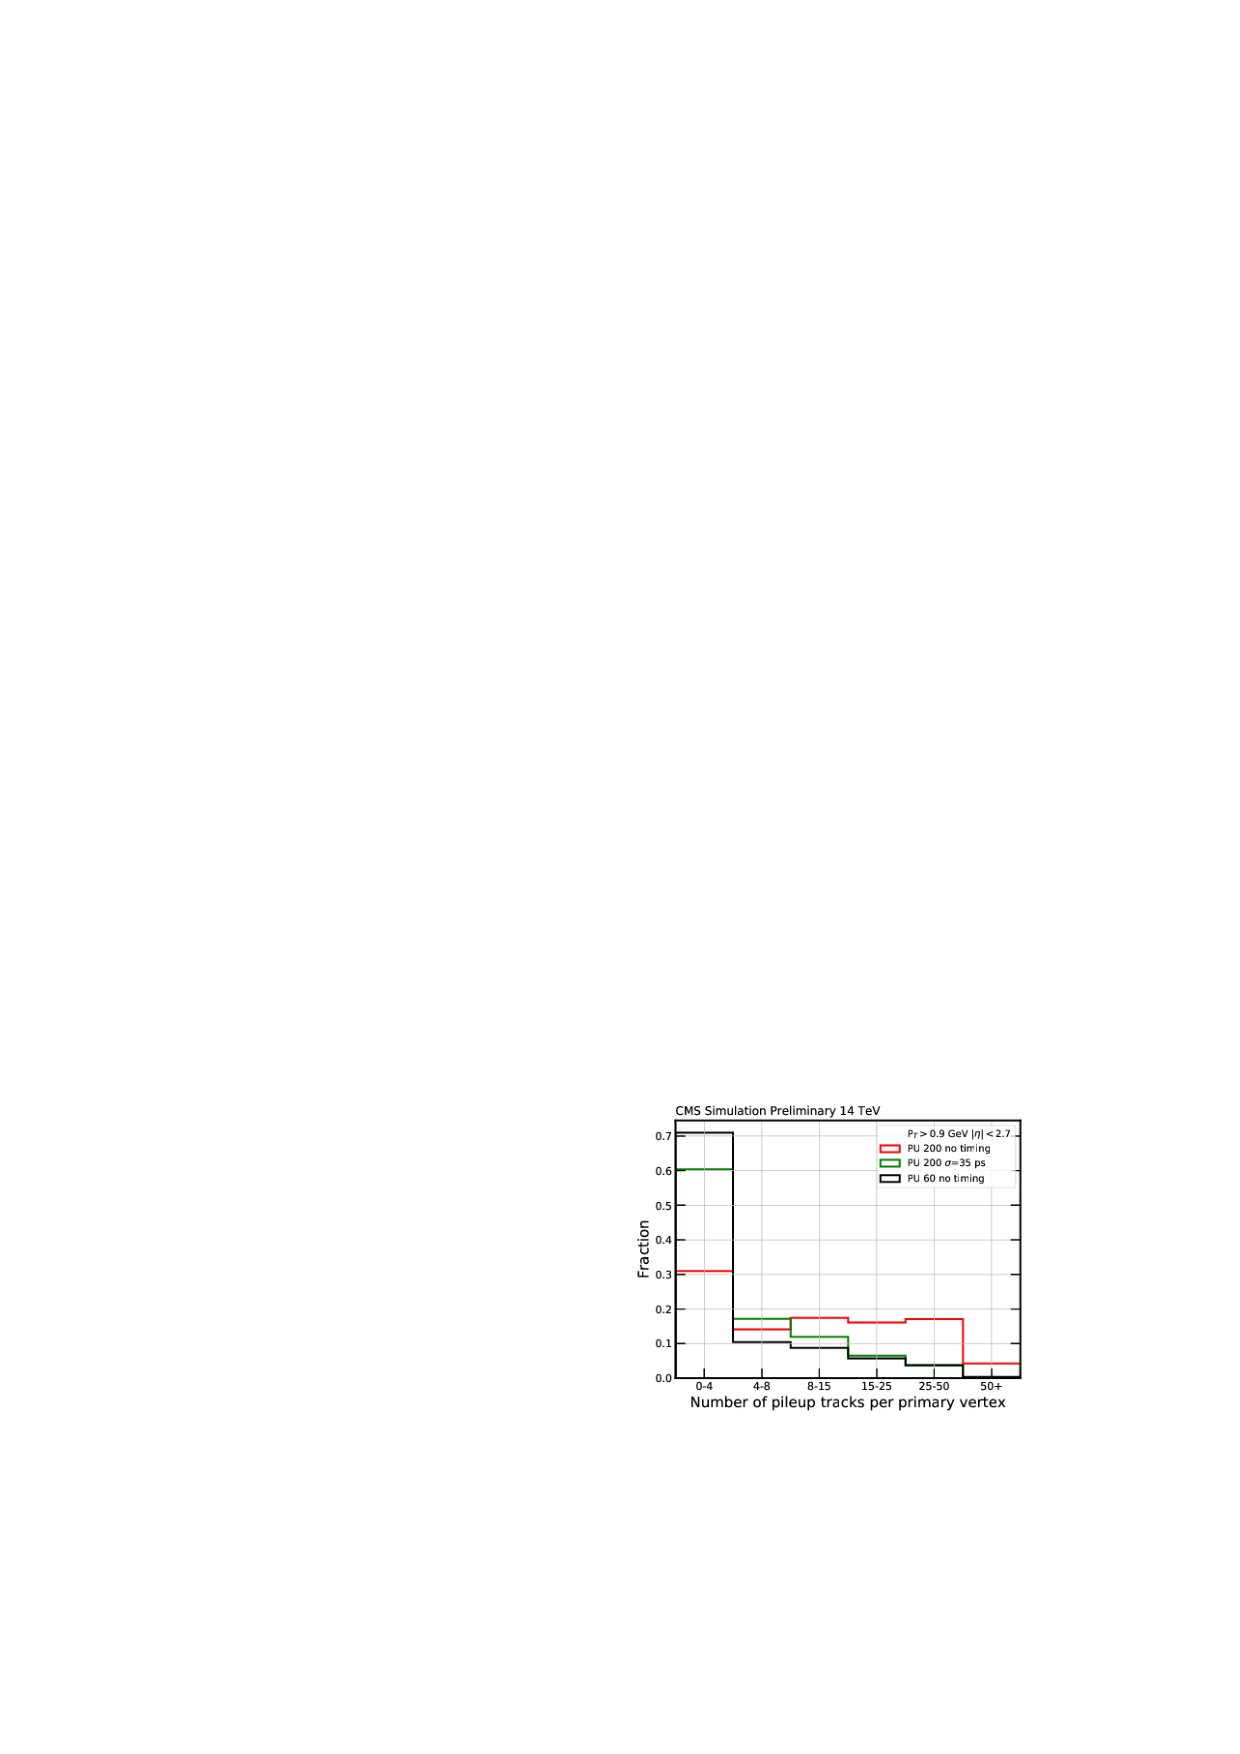
\includegraphics[width=.45\linewidth]{Dissertation/fig/pileup-reduce2.pdf}
}
\end{center}
\caption{Plots from the TDR\cite{cite-mtd-tdr} demonstrating pileup reduction from timing information. Left: Number of pileup tracks incorrectly associated with the hard interaction vertex as a function of the collision line density for different time resolutions. Right: Distribution of the number of incorrectly associated tracks with the use of a $3\sigma$ (where $\sigma = 35$ ps) selection on timing information and without use of timing information; the vertical axis is the fraction of primary vertices which have the number of pileup tracks shown on the horizontal axis
associated to them.}
\label{fig:pileup-reduce}
\end{figure}

\end{section}

\begin{section}{The Topolino Design}

The barrel and endcap layers (BTL and ETL respectively) of the MTD have rotational symmetries -- they are round -- while the sensors are rectangular, so some careful consideration is required when looking to cover the CMS detector with a new sensor layer. For the BTL, the design is fairly simple: long trays of sensors may be laid along the axis of the barrel, maintaining its cylindrical symmetry. However, correctly fitting the rectangular sensors to the circular space allotted on the endcaps (which are essentially annuli) becomes a complicated exercise in geometric optimization, while including space for all of the required circuitry, wiring, and cooling systems imposes complicated physical constraints.  Although the ETL offered unique complications, one design was arrived at -- named ``Topolino'' (Mickey Mouse in Italian) by its inventor -- where the ETL is divided into four ninety-degree wedges. The front of each wedge is tiled with parallel strips of sensors that continue up until the the edge of the endcap. The back of the same wedge is similarly covered, but the sensors are horizontally offset to cover the gaps left by the readout electronics on the front. Each wedge is covered in this way, then placed such that the sensors in each is perpendicular to its neighboring wedges. See Figure \ref{fig:topolino} for a detailed visualization of the proposed design.

\begin{figure}[htb]
\begin{center}
\subfloat[Rendered with no mounting disk to show coverage of electronics gaps.]      {
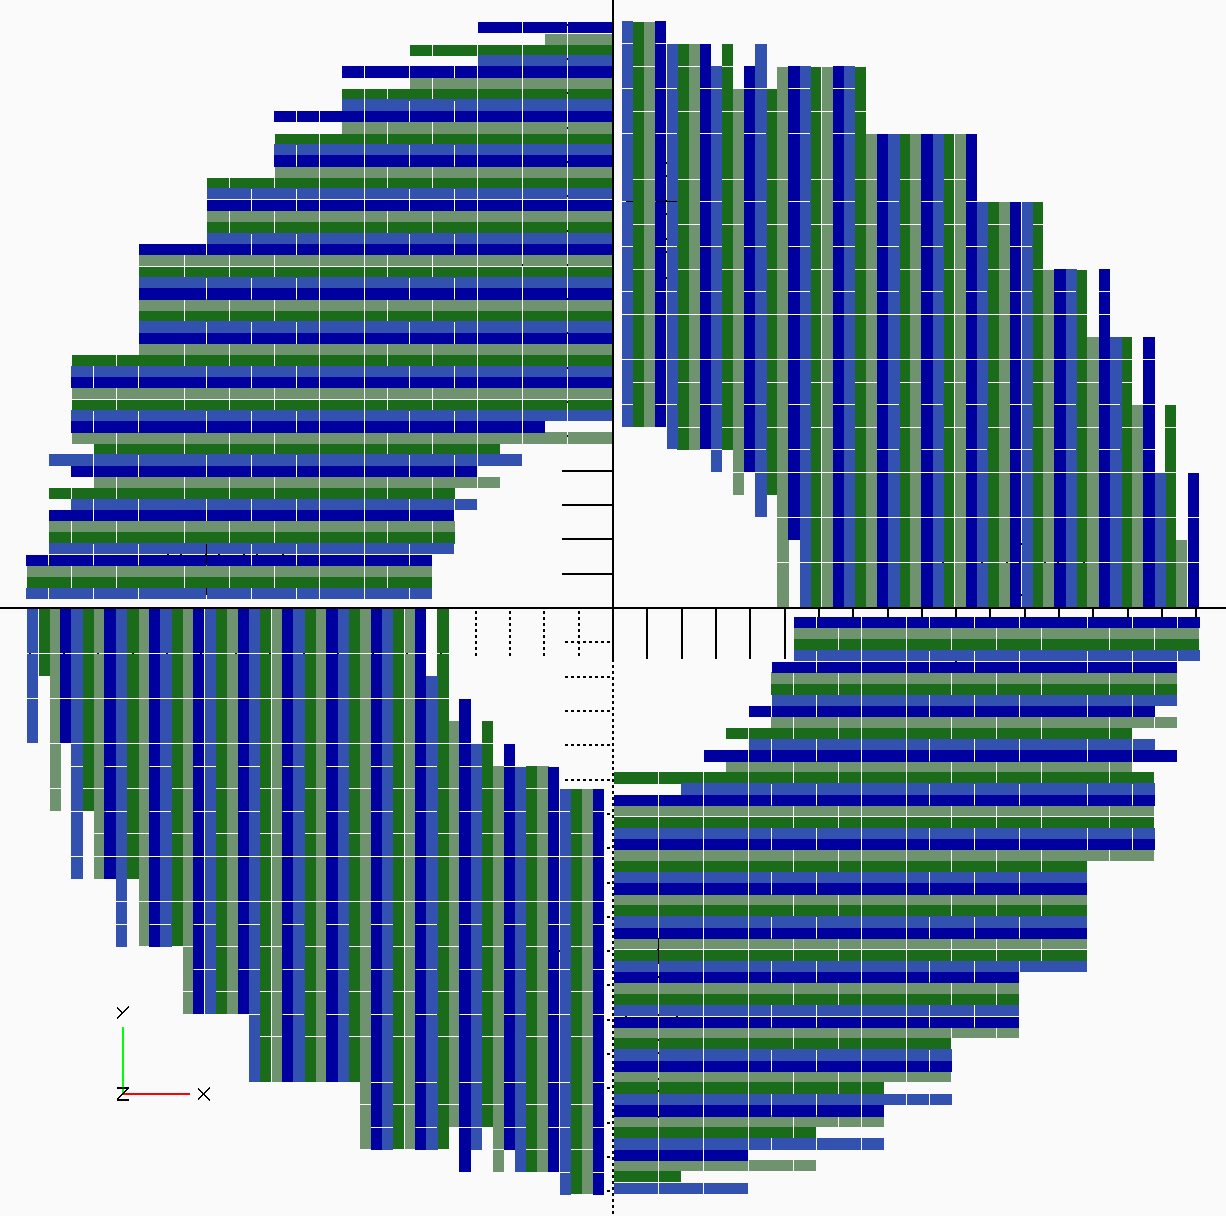
\includegraphics[width=.5\linewidth]{Dissertation/fig/topolino-nodisk.png}
}
\\
\subfloat[Front of one full disk.]      {
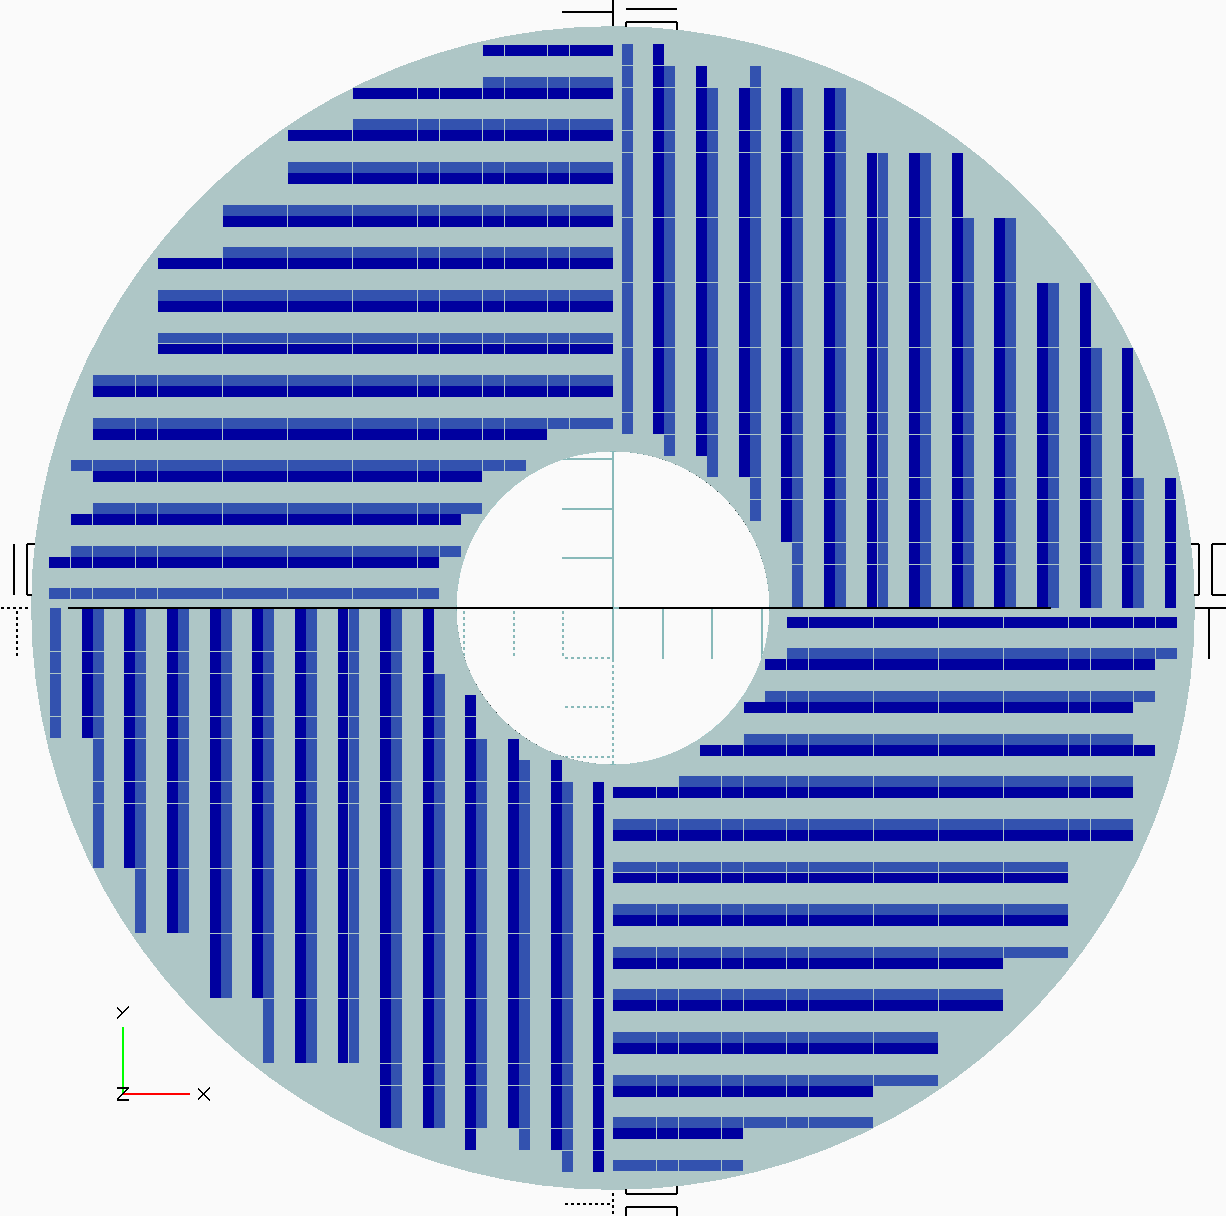
\includegraphics[width=.25\linewidth]{Dissertation/fig/topolino-front.png}
}\quad
\subfloat[Back of one full disk.]      {
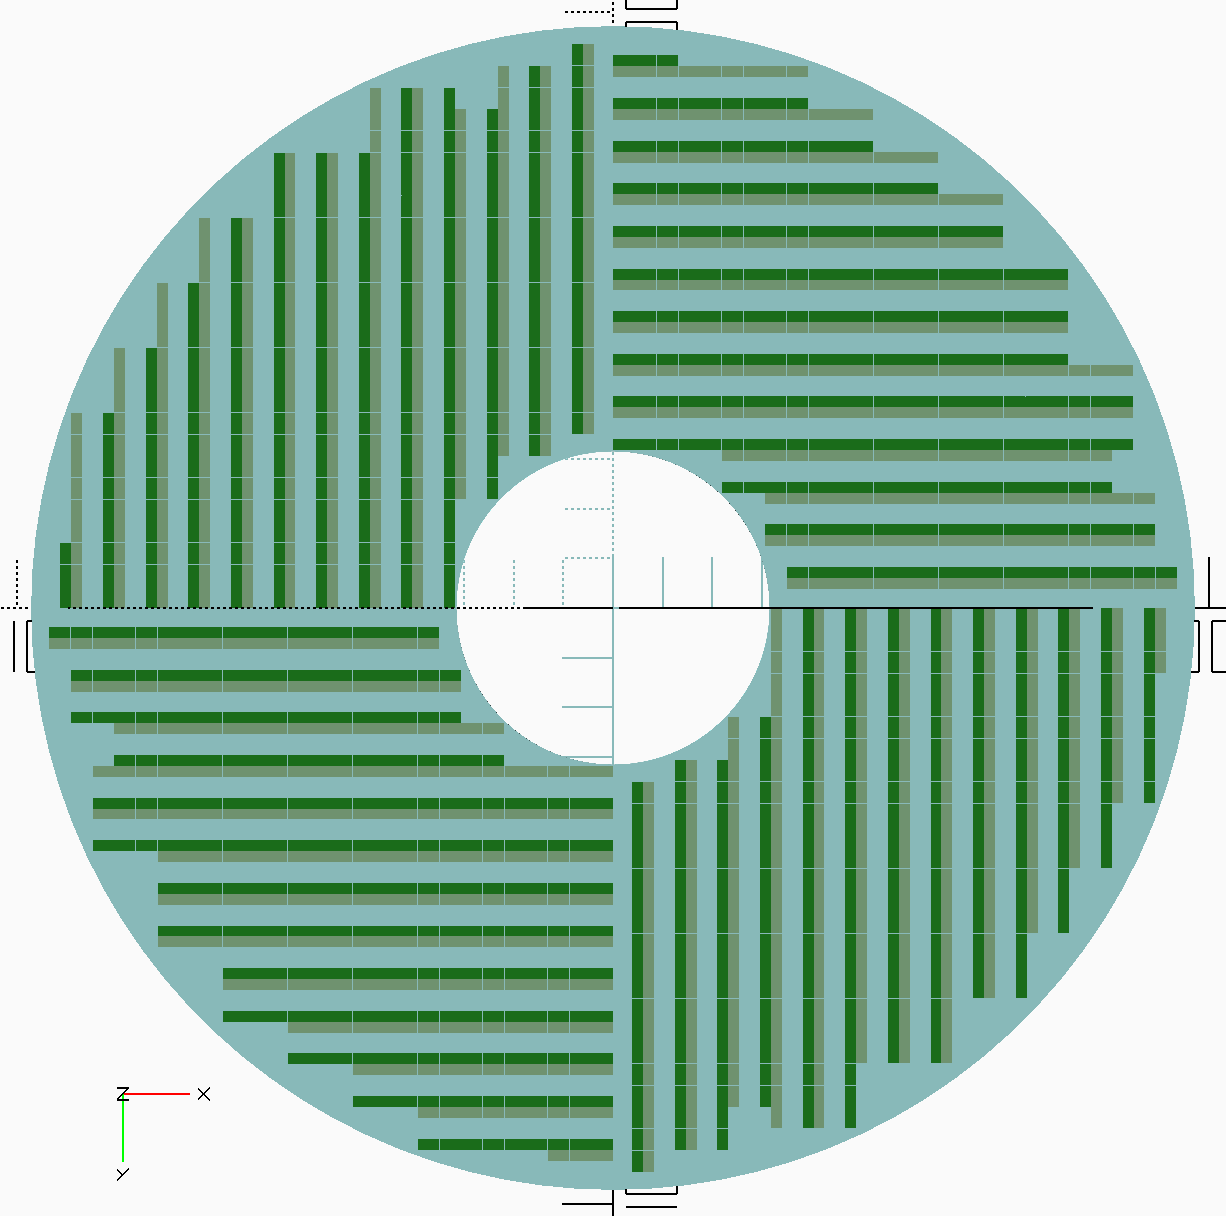
\includegraphics[width=.25\linewidth]{Dissertation/fig/topolino-back.png}
}
\end{center}
\caption{The ``topolino'' design.}
\label{fig:topolino}
\end{figure}

\end{section}

\begin{section}{Rendering the Detector}

Detector physics simulation begins with a simulation of the detector, but for answers to questions about the MTD's design and performance, verbose considerations of minute physical interactions are, at the moment, unnecessary. Therefore, though more complex tools offer more accurate physics, a simple rendering of each sensor's position is space is sufficient. However, the simulation must also be configurable, so assembling the it by hand, like most 3D-modeling software requires, was neither an entertaining, nor efficient solution. Instead, OpenSCAD, a C-like programming language that allows for simple, modular construction of three-dimensional models, was selected.

To algorithmically implement the Topolino design, fundamental rules that govern the layout had to be established. First, neither the sensors, nor the space allotted for their circuitry, could be allowed to hang over the perimeter of the endcap. Second, sensors are most easily assembled and placed as modules, so the detector must be tiled by \textit{groups} of sensors. Finally, the service modules -- the ``circuitry'' for which space has already been allotted -- are designed to service sensors on both sides, so sensors should (generally) be placed as such, resulting in a neat grid. With these rules in mind, an algorithm parses the x-axis in increments equal to the width of a sensor module, then places sensors by their lower, left-hand (closest to origin) corners, so long as their placement does not violate any of the previously stated rules. One wedge is tiled in this way where the sensors on its reverse side are placed in the same way but starting from a given displacement from the origin such that the holes left by the spacing for readout electronics are covered by sensors on the opposite side. The rest of the endcap is covered by simply taking this wedge, then placing orthogonally-rotated copies until the entire surface is covered. The images shown in Figure \ref{fig:topolino} were created by the algorithm described here.

\end{section}

\begin{section}{Simulating Performance}
\begin{subsection}{Pre-processing}
The three-dimensional model of the MTD can be exported as a Standard Tessellation Language (STL) file. During the export process, each independent object -- say, a single sensor which is represented as a thin rectangular prism -- is broken down into each of its constituent faces. Then, it undergoes the tessellation process, wherein the face considered is broken into some optimal number of constituent triangles (hereafter referred to as \textit{polygons}). The \textit{vertices} of each of these polygons are then written to the STL file, in a clockwise order relative to the origin. It is important to note that this guarantees that the \textit{facet normal} vector -- that is, a vector orthogonal to the surface of the polygon with a magnitude equal to the area of the polygon -- always points outwards with respect to the origin.
\end{subsection}
\begin{subsection}{Hit Detection Algorithm}
Now, before the simulation itself is generally discussed, the algorithm by which an intersection between a point and a polygon is determined should first be outlined, since it is the core operation of the simulation but is otherwise only tangentially important to the overall process. Consider a triangle in three-space, namely a set of three vectors $\vec{v}_1, \vec{v}_2, \vec{v}_3$ with facet normal $\hat{n}$, normalized such that $|\hat{n}| = 1$, pointing outwards relative to the origin. Then, suppose there exists a point $\vec{a}$ somewhere in three-space (see Figure \ref{fig:setup} for a visual representation of this setup). First, the coordinate system must be rotated into the plane of the polygon (in order to account for both the azimuthal symmetry of the BTL and radial symmetry of the ETL). One basis vector, arbitrarily chosen to be $\hat{e}_3'$, is already given by the facet normal vector. Another, now chosen to be $\hat{e}_{1}'$, is given by the original $\hat{e}_3$ vector (this is $\hat{z}$ is the CMS coordinate system; see Appendix \ref{appendix:cms-coords} for more information). With two basis vectors determined, the third is simply given by the cross product $\hat{e}_3'\times\hat{e}_1'$, assuming they are already normalized (again, see Figure \ref{fig:setup}). From this new set of basis vectors $\hat{e}_i'$, still represented in the original basis, a matrix $R$ can be constructed to translate any arbitrary vector into the primed coordinate system:

\begin{equation}
    \hat{e}_i' = \begin{pmatrix} x_i \\ y_i \\ z_i \end{pmatrix}
    \rightarrow
    R \equiv \begin{pmatrix} 
        x_1 & y_1 & z_1 \\
        x_2 & y_2 & z_2 \\
        x_3 & y_3 & z_3
    \end{pmatrix}
\end{equation}

\noindent The point $\vec{a}$ and vertices $\vec{v}_i$ are translated into the primed coordinate system such that $R\vec{a} = \vec{a}'$ and $R\vec{v}_i = \vec{v}_{i}'$. Then, the $\hat{e}_3'$ coordinates of $\vec{a}'$ and $\vec{v}_i'$ are set to zero, ensuring that all points considered are in the same plane parallel to that spanned by the polygon. Now, the vector from the point $\vec{a}'$ to the vertex $\vec{v}_{i}'$ is defined as $\vec{d}_{i}' \equiv \vec{v}_{i}'-\vec{a}'$. Finally, the following cross products are defined:

\begin{equation}
    \vec{C}_{i}' \equiv \epsilon_{ijk}(\vec{d}_{j}'\times\vec{d}_{k}')
\end{equation}

\noindent In words, the vectors $\vec{C}_{i}'$ are the cross products between adjacent vectors $\vec{d}_{j}'$, $\vec{d}_{k}'$ taken in cyclical permutations, as dictated by the Levi-Cevita symbol $\epsilon_{ijk}$. More importantly, however, each vector $\vec{C}_{i}'$ must be \textit{parallel} to the facet normal vector, which is $\hat{e}_{3}'$ in the primed coordinate system, if the point $\vec{a}$ lies \textit{inside} of the polygon. This is because the angles between each vector $\vec{d}_{i}'$ must add up to 180 degrees inside the polygon or 360 degrees outside by geometric constraint, so the angle between two vectors $\vec{d}_{i}'$, $\vec{d}_{j}'$ has an upper limit of 180 degrees inside of the triangle and 360 degrees outside. Thus, the cross product between these vectors will point one way (here, the positive $\hat{e}_3'$ direction) if the angle between them is less than 180 degrees or exactly anti-parallel (the $-\hat{e}_3'$ direction) otherwise, so if all $\vec{C}_{i}'$ are greater than zero, $\vec{a}$ must be inside of the polygon, otherwise, it can immediately determined that $\vec{a}$ is outside. Put concisely, point $\vec{a}$ intersects the polygon given by $\vec{v}_1, \vec{v}_2, \vec{v}_3$ and facet normal $\hat{n}$ if and only if $\vec{C}_{i}' > 0$ where $i\in[1,2,3]$.

\begin{figure}[htb]
\begin{center}

\subfloat[Original]      {
\tdplotsetmaincoords{60}{110}
\begin{tikzpicture}[scale=3,tdplot_main_coords]
 
  % variables
  % theta, phi for a
  \def\rvec{.8}
  \def\thetavec{30}
  \def\phivec{345}
  % theta, phi for v1
  \def\rvecone{1.0}
  \def\thetavecone{15}
  \def\phivecone{90}
  % theta, phi for v2
  \def\rvectwo{1.0}
  \def\thetavectwo{74}
  \def\phivectwo{54}
  % theta, phi for v3
  \def\rvecthree{0.8}
  \def\thetavecthree{74}
  \def\phivecthree{90}
  % theta, phi for n
  \def\rvecfour{.7}
  \def\thetavecfour{37}
  \def\phivecfour{72}
 
  % axes
  \coordinate (O) at (0,0,0);
  \draw[thick,->] (0,0,0) -- (1,0,0) node[anchor=north east]{$\hat{e}_1$};
  \draw[thick,->] (0,0,0) -- (0,1,0) node[anchor=north west]{$\hat{e}_2$};
  \draw[thick,->] (0,0,0) -- (0,0,1) node[anchor=south]{$\hat{e}_3$};
 
  % a
  \tdplotsetcoord{P}{\rvec}{\thetavec}{\phivec}
  \draw[-stealth,black] (O)  -- (P) node[above right] {$\vec{a}$};
  \draw[dashed,black]   (O)  -- (Pxy);
  \draw[dashed,black]   (P)  -- (Pxy);
  % n
  \tdplotsetcoord{N}{\rvecfour}{\thetavecfour}{\phivecfour}
  \draw[-stealth,black] (O)  -- (N) node[above right] {$\hat{n}$};
  \draw[dashed,black]   (O)  -- (Nxy);
  \draw[dashed,black]   (N)  -- (Nxy);
  % v1
  \tdplotsetcoord{A}{\rvecone}{\thetavecone}{\phivecone}
  \draw[-stealth,red] (O)  -- (A) node[above right] {$\vec{v}_1$};
  \draw[dashed,red]   (O)  -- (Axy);
  \draw[dashed,red]   (A)  -- (Axy);
  \draw[dashed,red]   (Ay) -- (Axy);
  % v2
  \tdplotsetcoord{B}{\rvectwo}{\thetavectwo}{\phivectwo}
  \draw[-stealth,green] (O)  -- (B) node[above right] {$\vec{v}_2$};
  \draw[dashed,green]   (O)  -- (Bxy);
  \draw[dashed,green]   (B)  -- (Bxy);
  \draw[dashed,green]   (By) -- (Bxy);
  % v3
  \tdplotsetcoord{C}{\rvecthree}{\thetavecthree}{\phivecthree}
  \draw[-stealth,blue] (O)  -- (C) node[above right] {$\vec{v}_3$};
  \draw[dashed,blue]   (O)  -- (Cxy);
  \draw[dashed,blue]   (C)  -- (Cxy);
  \draw[dashed,blue]   (Cy) -- (Cxy);
 
\end{tikzpicture}
}\quad
\subfloat[Primed]      {
\tdplotsetmaincoords{60}{110}
\begin{tikzpicture}[scale=3,tdplot_main_coords]
 
  % variables
  % theta, phi for a
  \def\rvec{.8}
  \def\thetavec{30}
  \def\phivec{345}
  % theta, phi for v1
  \def\rvecone{1.0}
  \def\thetavecone{15}
  \def\phivecone{90}
  % theta, phi for v2
  \def\rvectwo{1.0}
  \def\thetavectwo{74}
  \def\phivectwo{54}
  % theta, phi for v3
  \def\rvecthree{0.8}
  \def\thetavecthree{74}
  \def\phivecthree{90}
  % theta, phi for n
  \def\rvecfour{.7}
  \def\thetavecfour{37}
  \def\phivecfour{72}
  % theta, phi for e2
  \def\rvecfive{1.0}
  \def\thetavecfive{-53}
  \def\phivecfive{90}
 
  % axes
  \coordinate (O) at (0,0,0);
  \draw[thick,->] (0,0,0) -- (1,0,0) node[anchor=north east]{$\hat{e}_{1}'$};
  \tdplotsetcoord{E}{\rvecfive}{\thetavecfive}{\phivecfive}
  \draw[thick,->] (0,0,0) -- (E) node[anchor=north west]{$\hat{e}_{2}'$};
  \tdplotsetcoord{E}{\rvecfour}{\thetavecfour}{\phivecfour}
  \draw[thick,->] (0,0,0) -- (E) node[anchor=south]{$\hat{e}_{3}'$};
 
  % a
  \tdplotsetcoord{P}{\rvec}{\thetavec}{\phivec}
  \draw[-stealth,black] (O)  -- (P) node[above right] {$\vec{a}$};
  \draw[dashed,black]   (O)  -- (Pxy);
  \draw[dashed,black]   (P)  -- (Pxy);
  % v1
  \tdplotsetcoord{A}{\rvecone}{\thetavecone}{\phivecone}
  \draw[-stealth,red] (O)  -- (A) node[above right] {$\vec{v}_1$};
  \draw[dashed,red]   (O)  -- (Axy);
  \draw[dashed,red]   (A)  -- (Axy);
  \draw[dashed,red]   (Ay) -- (Axy);
  % v2
  \tdplotsetcoord{B}{\rvectwo}{\thetavectwo}{\phivectwo}
  \draw[-stealth,green] (O)  -- (B) node[above right] {$\vec{v}_2$};
  \draw[dashed,green]   (O)  -- (Bxy);
  \draw[dashed,green]   (B)  -- (Bxy);
  \draw[dashed,green]   (By) -- (Bxy);
  % v3
  \tdplotsetcoord{C}{\rvecthree}{\thetavecthree}{\phivecthree}
  \draw[-stealth,blue] (O)  -- (C) node[above right] {$\vec{v}_3$};
  \draw[dashed,blue]   (O)  -- (Cxy);
  \draw[dashed,blue]   (C)  -- (Cxy);
  \draw[dashed,blue]   (Cy) -- (Cxy);
 
\end{tikzpicture}
}

\end{center}
\caption{Coordinate systems used.}
\label{fig:setup}
\end{figure}

\begin{figure}[htb]
\begin{center}

\subfloat[Inside]      {
\tdplotsetmaincoords{60}{110}
\begin{tikzpicture}[scale=3,tdplot_main_coords]
 
  % variables
  % theta, phi for v1
  \def\rvecone{1.0}
  \def\thetavecone{90}
  \def\phivecone{90}
  % theta, phi for v2
  \def\rvectwo{1.0}
  \def\thetavectwo{90}
  \def\phivectwo{54}
  % theta, phi for v3
  \def\rvecthree{0.8}
  \def\thetavecthree{90}
  \def\phivecthree{270}
 
  % axes
  \coordinate (O) at (0.2,-0.3,0);
  \draw[thick,->] (0,0,0) -- (1,0,0) node[anchor=north east]{$\hat{e}_1'$};
  \draw[thick,->] (0,0,0) -- (0,1,0) node[anchor=north west]{$\hat{e}_2'$};
  \draw[thick,->] (0,0,0) -- (0,0,1) node[anchor=south]{$\hat{e}_3'$};

  \draw plot [mark=*, mark size=0.5] coordinates{(0.2,-0.3,0)};
  % a
  \draw[-stealth,black] (0,0,0) -- (0.2,-0.3,0) node[above right]{$\vec{a}'$};
  % d1
  \tdplotsetcoord{A}{\rvecone}{\thetavecone}{\phivecone}
  \draw[-stealth,red] (O)  -- (A) node[above right] {$\vec{d}_{1}'$};
  % d2
  \tdplotsetcoord{B}{\rvectwo}{\thetavectwo}{\phivectwo}
  \draw[-stealth,green] (O)  -- (B) node[above right] {$\vec{d}_{2}'$};
  % d3
  \tdplotsetcoord{C}{\rvecthree}{\thetavecthree}{\phivecthree}
  \draw[-stealth,blue] (O)  -- (C) node[above right] {$\vec{d}_{3}'$};
  % d3->d1
  \tdplotdrawarc[thick,->]{(O)}{0.4}{246}{99}
  {anchor=north}{};
  % d1->d2
  \tdplotdrawarc[thick,->]{(O)}{0.4}{99}{68}
  {anchor=north}{};
  % d2->d3
  \tdplotdrawarc[thick,->]{(O)}{0.4}{68}{-114}
  {anchor=north}{};
 
\end{tikzpicture}
}\quad
\subfloat[Outside]      {
\tdplotsetmaincoords{60}{110}
\begin{tikzpicture}[scale=3,tdplot_main_coords]
 
  % variables
  % theta, phi for v1
  \def\rvecone{1.0}
  \def\thetavecone{90}
  \def\phivecone{90}
  % theta, phi for v2
  \def\rvectwo{1.0}
  \def\thetavectwo{90}
  \def\phivectwo{54}
  % theta, phi for v3
  \def\rvecthree{0.8}
  \def\thetavecthree{90}
  \def\phivecthree{270}
 
  % axes
  \coordinate (O) at (-0.75,0,0);
  \draw[thick,->] (0,0,0) -- (1,0,0) node[anchor=north east]{$\hat{e}_1'$};
  \draw[thick,->] (0,0,0) -- (0,1,0) node[anchor=north west]{$\hat{e}_2'$};
  \draw[thick,->] (0,0,0) -- (0,0,1) node[anchor=south]{$\hat{e}_3'$};

  \draw plot [mark=x, mark size=1] coordinates{(-0.75,0,0)};
  % a
  \draw[-stealth,black] (0,0,0) -- (-0.75,0,0) node[above right]{$\vec{a}'$};
  % d1
  \tdplotsetcoord{A}{\rvecone}{\thetavecone}{\phivecone}
  \draw[-stealth,red] (O)  -- (A) node[above right] {$\vec{d}_{1}'$};
  % d2
  \tdplotsetcoord{B}{\rvectwo}{\thetavectwo}{\phivectwo}
  \draw[-stealth,green] (O)  -- (B) node[above right] {$\vec{d}_{2}'$};
  % d3
  \tdplotsetcoord{C}{\rvecthree}{\thetavecthree}{\phivecthree}
  \draw[-stealth,blue] (O)  -- (C) node[above right] {$\vec{d}_{3}'$};
  % d3->d1
  \tdplotdrawarc[thick,->,dashed]{(O)}{0.5}{311}{54}
  {anchor=north}{};
  % d1->d2
  \tdplotdrawarc[thick,->]{(O)}{0.5}{54}{30}
  {anchor=north}{};
  % d2->d3
  \tdplotdrawarc[thick,->]{(O)}{0.5}{30}{-51}
  {anchor=north}{};
 
\end{tikzpicture}
}

\end{center}
\caption{Illustration of vectors from hit position to vertices.}
\label{fig:vectors}
\end{figure}

\end{subsection}
\begin{subsection}{Post-processing}
The STL representation of the MTD and a text file containing the kinematics of many thousands of simulated particle trajectories is now input to a Python program that operates as follows: for each trajectory in the trajectory file, parse over every polygon in the STL file and check if the trajectory intersects the polygon using the algorithm described previously; if intersection, save some kinematics of the trajectory including the hit position; else, continue. This is, in essence, how many ``ray tracing'' algorithms function\cite{raytrace}, which calculate effects like lighting for computer graphics. Ray tracing is a slow process, which is why graphics seen in movies are pre-rendered and far more detailed and realistic than graphics computed in real time, though recent developments are making real-time, brute-force ray tracing more feasible. However, such technology was neither present nor necessary for this simulation. Instead, the Condor\cite{condor} system on the Tier 2 computing center at UC San Diego was used to run the algorithm over approximately 250,000 trajectories. As a result, plots accurate up to the millimeter scale may be produced to study the efficiency of the entire MTD for a dynamic range of geometries. An example of the simulation's output is shown in Figure \ref{fig:chronoplots}.

\begin{figure}[htb]
\begin{center}
\subfloat[]      {
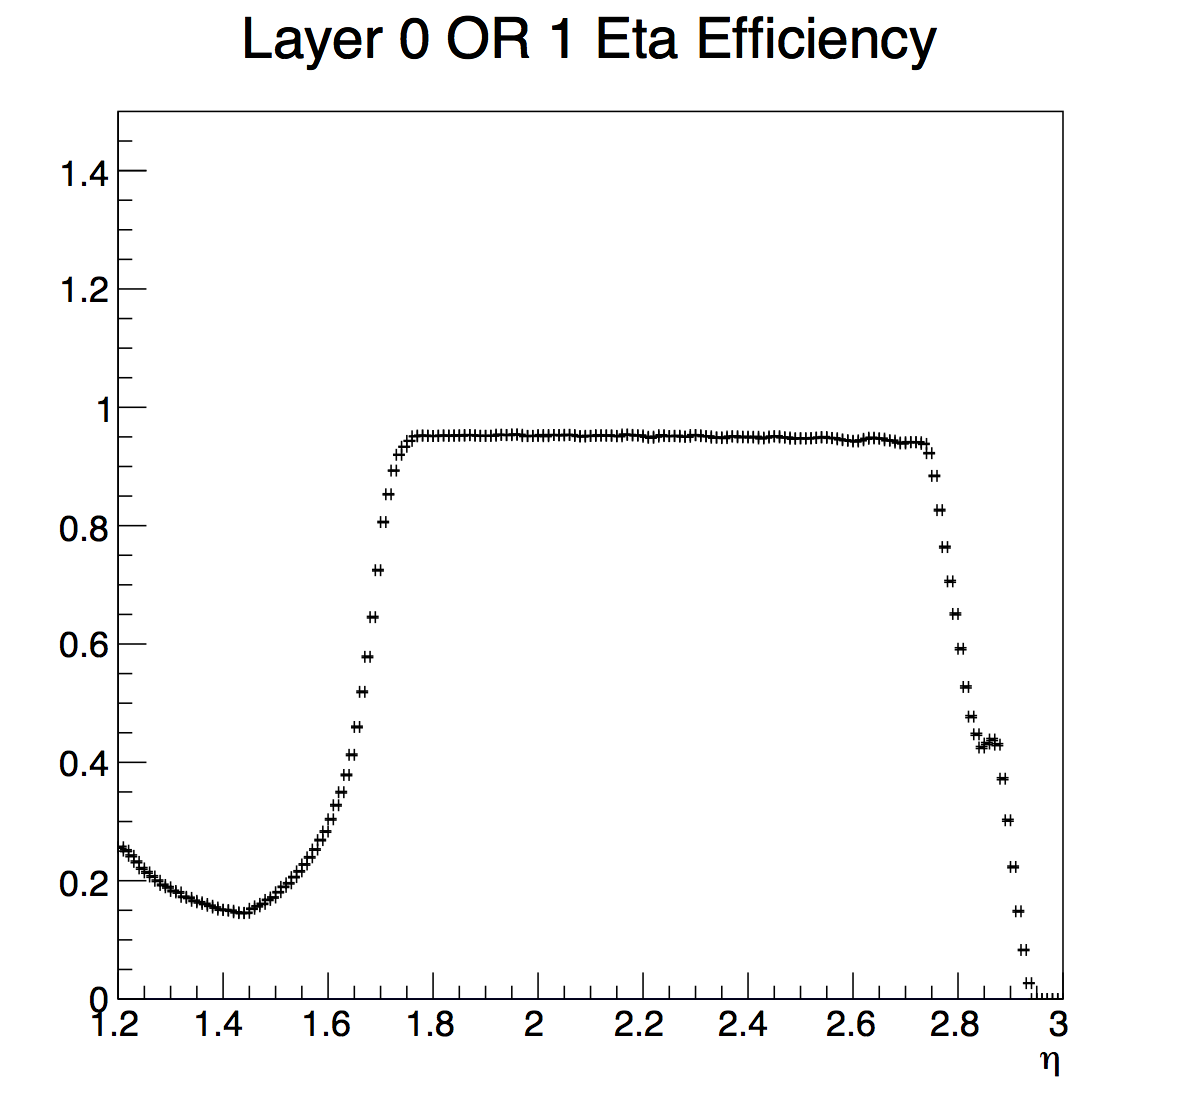
\includegraphics[width=.25\linewidth]{Dissertation/fig/DiskEtaEff01-1190mm.png}
}\quad
\subfloat[]      {
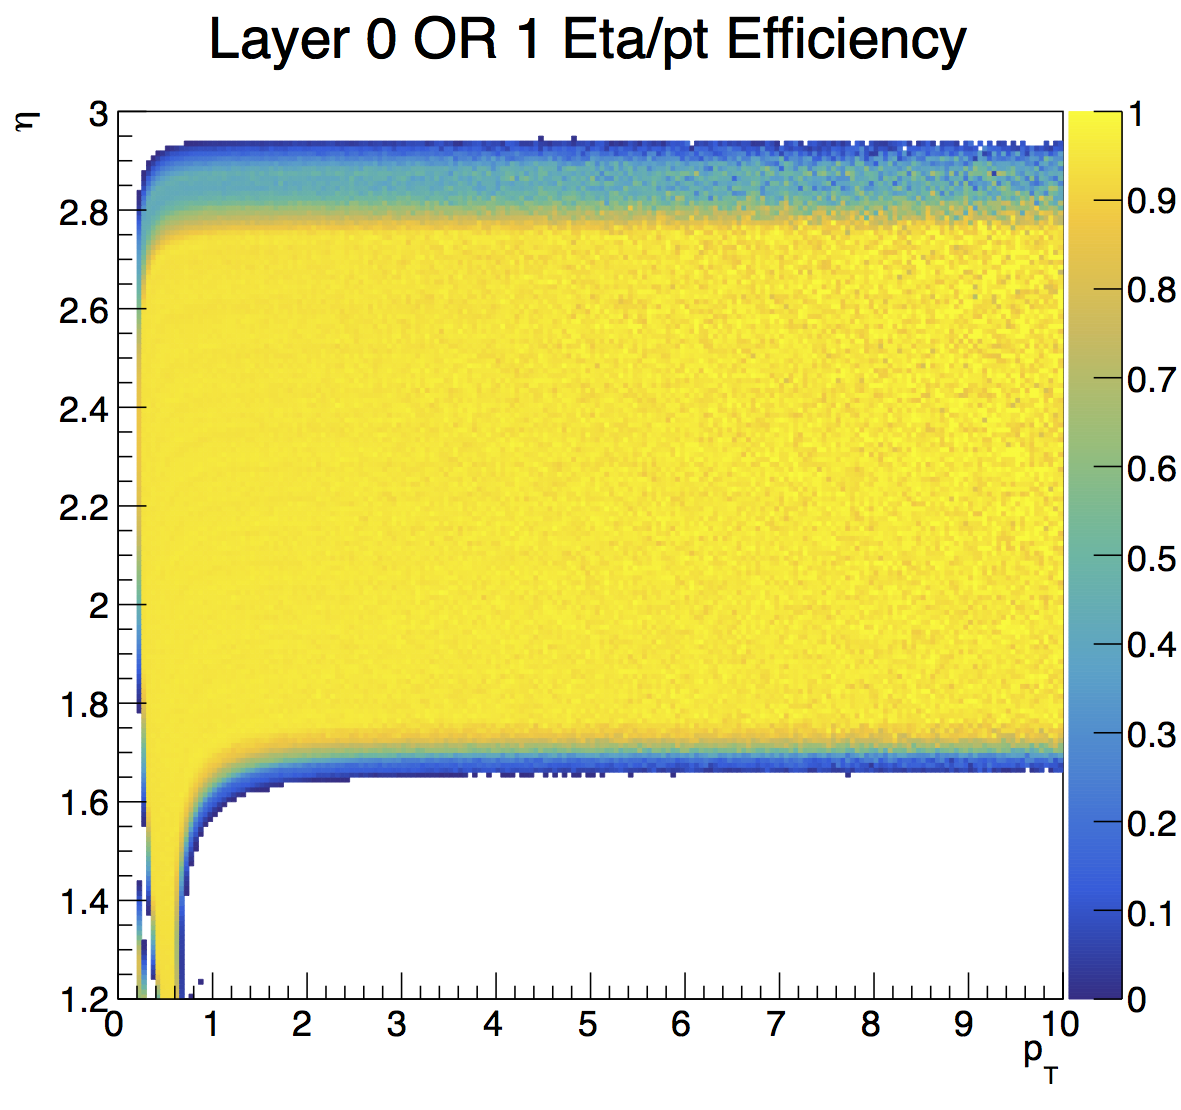
\includegraphics[width=.25\linewidth]{Dissertation/fig/DiskEtaPtEff01-1190mm.png}
}\\
\subfloat[]      {
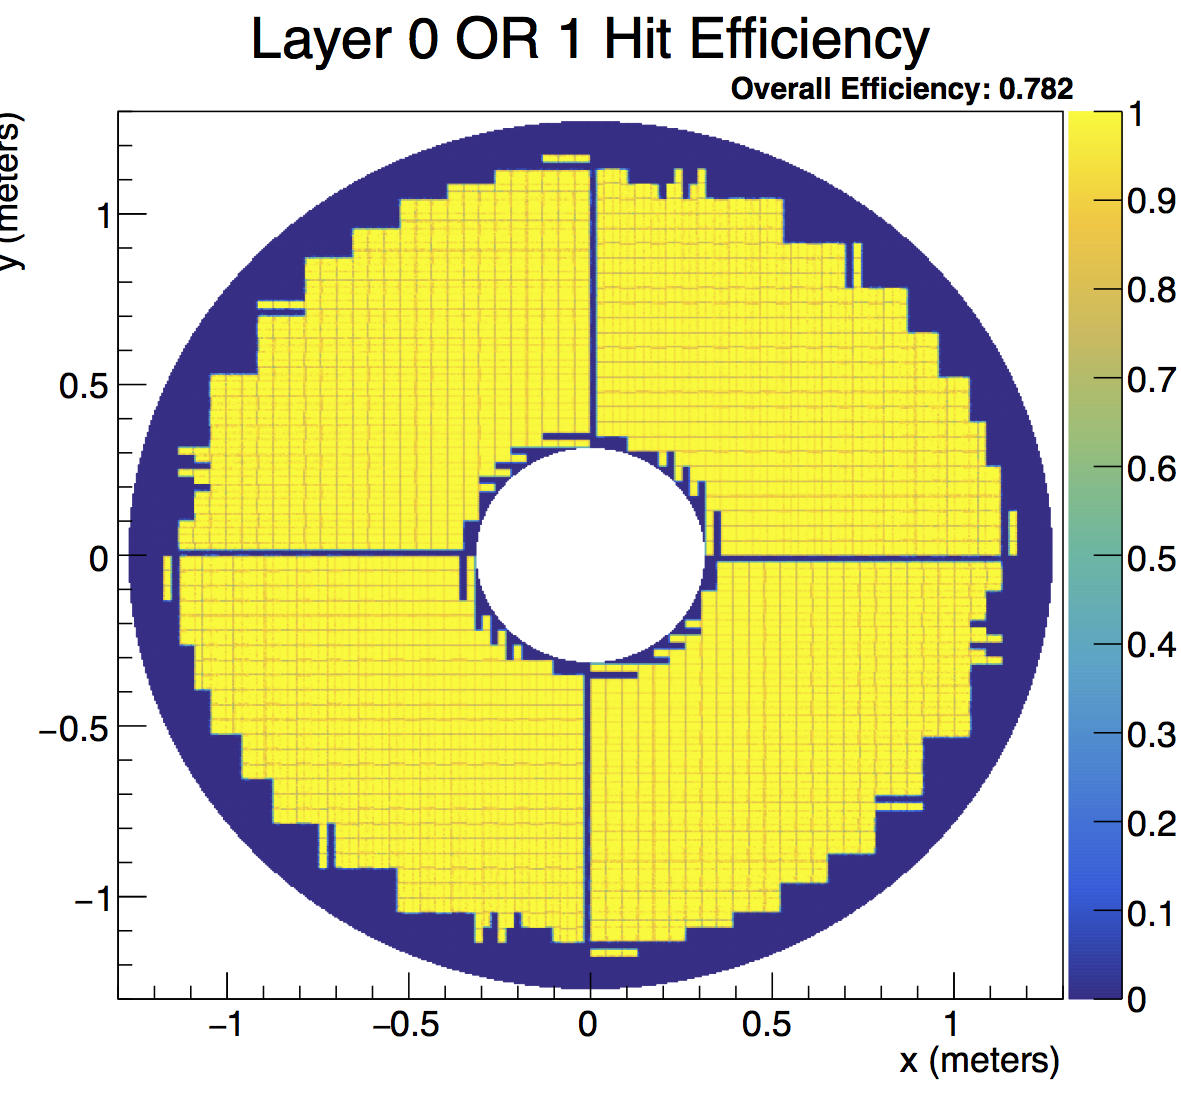
\includegraphics[width=.25\linewidth]{Dissertation/fig/LayerHitEff01-1190mm.png}
}\quad
\subfloat[]      {
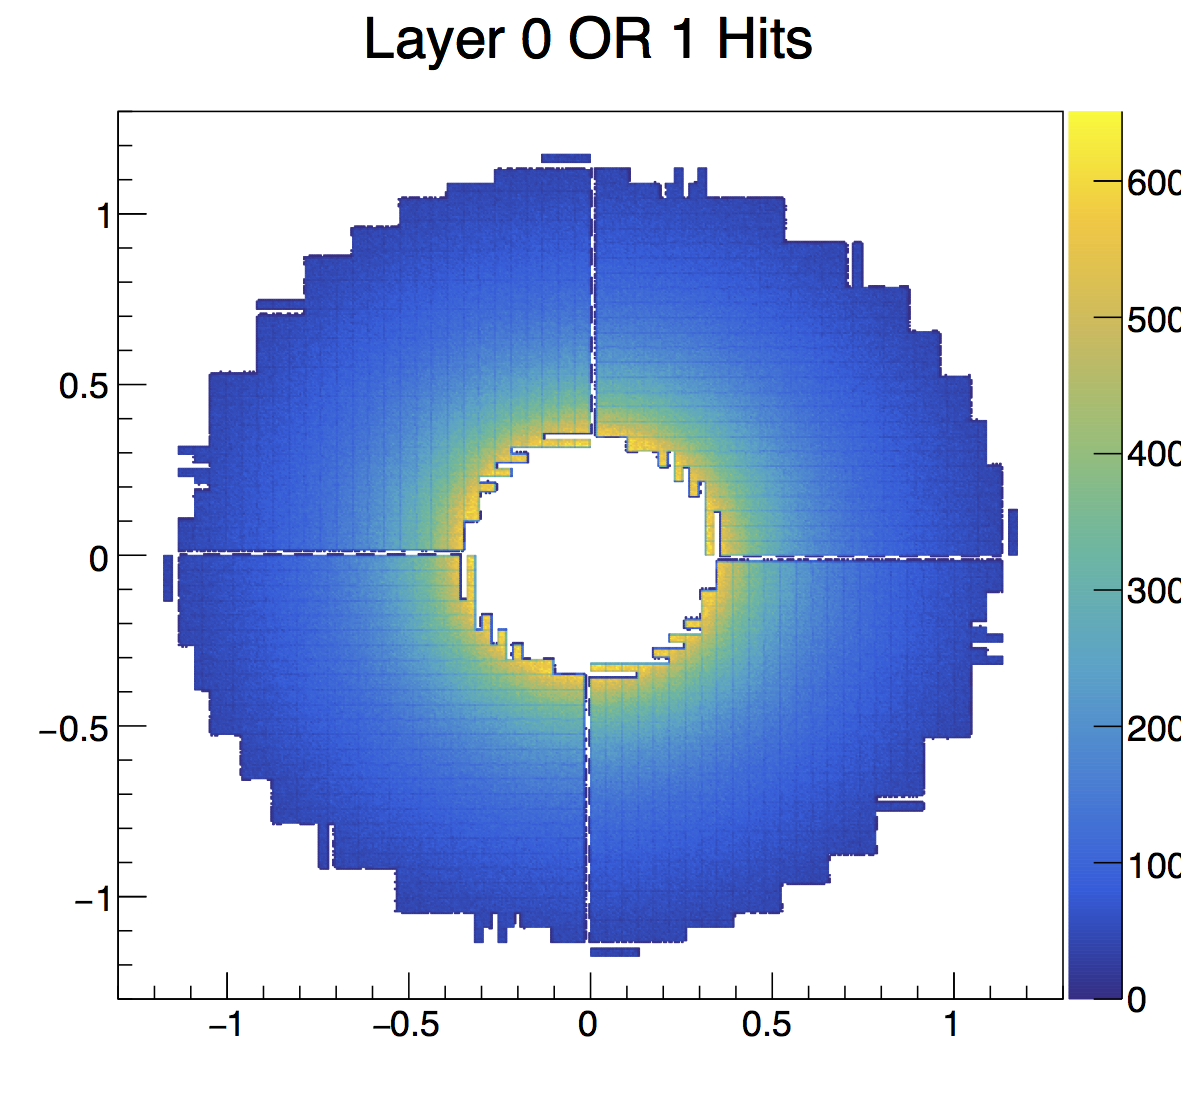
\includegraphics[width=.25\linewidth]{Dissertation/fig/LayerHits01-1190mm.png}
}
\end{center}
\caption{Efficiency plots produced using simulation data for the ETL with a 1190mm outer radius and 315mm inner radius following the Topolino design.}
\label{fig:chronoplots}
\end{figure}

\end{subsection}
\end{section}

%=== Chapter 3  ============================================
\chapter{Measurement of Rare Higgs Decays}
%
%  Search for Rare Higgs Decays
%

I begin with a brief discussion of the motivation behind looking for rare Higgs decays like $H \rightarrow \rho+\gamma$ and $H \rightarrow \phi+\gamma$, specifically via the associated $WH$ rather than direct production. Then, I outline the event selection methods and relevant backgrounds. Finally, I describe the Boosted Decision tree we used in detail, followed by the results of the analysis.

\begin{section}{Motivation}

The branching ratios for the $H \rightarrow \phi+\gamma$ and $H \rightarrow \rho+\gamma$ decays are expected to have a lower bound of $8.8 \times 10^{-4}$ and $4.8 \times 10^{-4}$  respectively\cite{cite-rpg-brs}. Put simply, they are \textit{very} rare - so rare, in fact, that they have never been directly observed. Furthermore, by any measure, these decays should never be detectable at current, human-reachable energies, that is, unless there are yet-undiscovered processes that enhance the rate of either of these decays. This implies that this measurement is experimentally exciting, because any significant measurement of the production of $\rho$ or $\phi$ mesons would be direct evidence of the existence of new physics. At the same time, if no $\rho$ or $\phi$ mesons are found, then the branching ratio of either decay mode can be pushed farther back, depending on the detector's sensitivity to the signature.

Now, ideally, we would search for these decays via \textit{direct} production, that is, when a Higgs boson is produced by gluon-gluon fusion (Fig. \ref{fig:direct-prod}), then decays to a photon and a $\phi$ or $\rho$ meson. However, CMS does not have a dedicated trigger for detecting pions or kaons (the final-state products of the $\phi$ and $\rho$ mesons respectively), so the only possibly detectable particle would be the photon. However, since the Higgs mass is 125 GeV, the photon and meson both have a momentum of approximately 60 GeV at most, so the photon is well below the threshold of the CMS single photon trigger\cite{cite-hlt}. Therefore, we chose an associate production mode, namely, $W^{\pm}+H$ (Fig. \ref{fig:whiggs-prod}), where $W \rightarrow \ell^{\pm}+\nu_{\ell}$. We can easily trigger on the leptons produced by the $W$ boson, and the Higgs comes for free. At the same time, we lose a \textit{lot} of signal, since this process is far more rare. We also have to deal with more background, since we are including more particles in the signature we are searching for. Ultimately these consequences consolidate into an overall loss of sensitivity, but alternative associated productions ($Z+H$, for instance) face similar challenges.

\begin{figure}[htb]
\begin{center}
% Naming convention:
%    <above/below : a/b><level: #>_<#cm from origin>
%    Examples:
%       a2_0 = above, level 2, at origin
%       b3_1 = below, level 3, 1cm from origin

\begin{tikzpicture}
  \begin{feynman}
    
    % START: Horizon ---------------------------------
    \vertex (horizon);
    \vertex[right=5cm of horizon] (hz_5);
    \vertex[right=7cm of horizon] (hz_7);
    % END: Horizon -----------------------------------
    
    % START: Above -----------------------------------
    % Level +3
    \vertex[above=3cm of horizon] (a3);
    \vertex[right=13cm of a3] (a3_13) {\(u,s\)};
    % Level +2
    \vertex[above=2cm of horizon] (a2);
    \vertex[left=1cm of a2] (1_a2) {\(g\)};
    \vertex[right=2cm of a2] (a2_2);
    \vertex[right=10cm of a2] (a2_10);
    \vertex[right=12cm of a2] (a2_12);
    % Level +1
    \vertex[above=1cm of horizon] (a1);
    \vertex[right=13cm of a1] (a1_13) {\(\overline u,\overline s\)};
    % END: Above -------------------------------------
    
    % START: Below -----------------------------------
    % Level -2
    \vertex[below=2cm of horizon] (b2);
    \vertex[left=1cm of b2] (1_b2) {\(g\)};
    \vertex[right=2cm of b2] (b2_2);
    \vertex[right=10cm of b2] (b2_10);
    \vertex[right=13cm of b2] (b2_13) {\(\gamma\)};

    \diagram* {
      {[edges=gluon]
        (1_a2) -- (a2_2),
        (1_b2) -- (b2_2),
      },
      
      (a2_2) -- [fermion, edge label=\(t\)] (hz_5),
      (b2_2) -- [anti fermion, edge label=\(\overline t\)] (hz_5),
      (a2_2) -- [anti fermion, edge label=\(\overline t\)] (b2_2),
      
      (hz_5) -- [scalar, edge label=\(H\)] (hz_7),
      
      (hz_7) -- [fermion, edge label=\(t\)] (a2_10),
      (b2_10) -- [anti fermion, edge label=\(\overline t\)] (a2_10),
      (hz_7) -- [anti fermion, edge label=\(\overline t\)] (b2_10),
      
      (a2_10) -- [photon, edge label=\(\gamma\)] (a2_12),
      (a2_12) -- [fermion] (a3_13),
      (a2_12) -- [anti fermion] (a1_13),
      
      (b2_10) -- [photon] (b2_13),
    };
    
    \draw [decoration={brace}, decorate] (a3_13.north east) -- (a1_13.south east)
          node [pos=0.5, right] {\(\rho, \phi\)};
  \end{feynman}
\end{tikzpicture}
\end{center}
\caption{Feynman diagram\cite{cite-tikz-feynman} for primary mechanism of the direct production of the Higgs boson at the LHC where $H \rightarrow \rho+\gamma$ or $H \rightarrow \phi+\gamma$.}
\label{fig:direct-prod}
\end{figure}

\begin{figure}[htb]
\begin{center}
% Naming convention:
%    <above/below : a/b><level: #>_<#cm from origin>
%    Examples:
%       a2_0 = above, level 2, at origin
%       b3_1 = below, level 3, 1cm from origin

\begin{tikzpicture}
  \begin{feynman}
    
    % START: Horizon ---------------------------------
    \vertex (horizon);
    \vertex[right=1cm of horizon] (hz_1);
    \vertex[right=3cm of horizon] (hz_3);
    \vertex[right=9cm of horizon] (hz_9) {\(u,s\)};
    % END: Horizon -----------------------------------
    
    % START: Above -----------------------------------
     % Level +3
    \vertex[above=3cm of horizon] (a3_0);
    \vertex[right=6cm of a3_0] (a3_7) {\(\ell^{\pm}\)};
    % Level +2
    \vertex[above=2cm of horizon] (a2_0);
    \vertex[right=5cm of a2_0] (a2_5);
    % Level +1
    \vertex[above=1cm of horizon] (a1_0);
    \vertex[left=1cm of a1_0] (a1_1) {\(q\)};
    \vertex[right=6cm of a1_0] (a1_7) {\(\nu_{\ell}\)};
    % END: Above -------------------------------------
    
    % START: Below -----------------------------------
    % Level -1
    \vertex[below=1cm of horizon] (b1_0);
    \vertex[left=1cm of b1_0] (b1_1) {\(\overline q\)};
    \vertex[right=7cm of b1_0] (b1_7);
    \vertex[right=8cm of b1_0] (b1_8);
    % Level -2
    \vertex[below=2cm of horizon] (b2_0);
    \vertex[right=5cm of b2_0] (b2_5);
    \vertex[right=9cm of b2_0] (b2_9) {\(\overline u,\overline s\)};
    % Level -3
    \vertex[below=3cm of horizon] (b3_0);
    \vertex[right=7cm of b3_0] (b3_7);
    \vertex[right=9cm of b3_0] (b3_9) {\(\gamma\)};

    \diagram* {
      (a1_1) -- [fermion, edge] (hz_1),
      (b1_1) -- [anti fermion, edge] (hz_1),
      
      (hz_1) -- [boson, edge label=\(W^{*}\)] (hz_3),
      (hz_3) -- [boson, edge label=\(W^{\pm}\)] (a2_5),
      (hz_3) -- [scalar, edge label=\(H\)] (b2_5),
      
      {[edges=fermion]
        (a2_5) -- (a3_7),
        (a2_5) -- (a1_7),
      },
      
      (b2_5) -- [fermion, edge label=\(t\)] (b1_7),
      (b1_7) -- [fermion, edge label=\(t\)] (b3_7),
      (b2_5) -- [anti fermion, edge label=\(\overline t\)] (b3_7),
      
      (b1_7) -- [photon, edge label=\(\gamma\)] (b1_8),
      (b3_7) -- [photon] (b3_9),
      
      (b1_8) -- [fermion, edge] (hz_9),
      (b1_8) -- [anti fermion, edge] (b2_9),
    };
    
    \draw [decoration={brace}, decorate] (hz_9.north east) -- (b2_9.south east)
          node [pos=0.5, right] {\(\rho, \phi\)};
  \end{feynman}
\end{tikzpicture}
\end{center}
\caption{Feynman diagram\cite{cite-tikz-feynman} for primary mechanism of the associated $WH$ production at the LHC studied in this analysis.}
\label{fig:whiggs-prod}
\end{figure}
\end{section}

\begin{section}{Event Selection}
\begin{subsection}{Data Aquisition}
The analysis begins with data based on a sample of proton-proton collisions collected by the Compact Muon Solenoid (CMS) detector in the LHC. ``Interesting'' events are selected by the first level of the CMS trigger system which uses information from the detector's calorimeters and muon detectors to select events for analysis in a fixed time interval of less than 4 $\mu s$. These events are then further processed by a high-level trigger processor farm, which decreases the event rate from around 100 kHz to less than 1 kHz, before the data is stored. Finally, the particle-flow algorithm reconstructs and identifies all particles from the events selected by the CMS trigger system. With the data properly processed and promptly reconstructed ``online,'' further analysis can be carried out ``offline.''
\end{subsection}
\begin{subsection}{Baseline Selection}
To start offline analysis, we first apply a baseline selection on data and Monte Carlo samples to filter out particularly irrelevant events. First, we require at one ``good" lepton, qualified as:
\begin{itemize}
    \item $p_{T}(\ell^{\pm}) > 10\textnormal{ GeV}$
    \item $\eta(\ell^{\pm}) < 2.4$
    \item $ID(e^{\pm})$ \verb|HAD_medium_noiso_v5|
    \item $ID(\mu^{\pm})$ \verb|isMediumMuonPOG|
    \item $I_{rel}(e^{\pm}) < 0.1$ using \verb|elMiniRelIsoCMS3_EA|
    \item $I_{rel}(\mu^{\pm}) < 0.2$ using \verb|muMiniRelIsoCMS3_EA|
\end{itemize}

\noindent We also require one good photon, qualified as:
\begin{itemize}
    \item $p_{T}(\gamma) > 20\textnormal{ GeV}$
    \item $\eta(\gamma) < 2.5$
    \item $ID(\gamma)$ \verb|isMediumPhotonPOG_Fall17V2|
    \item $I_{rel}(\gamma) < 0.06$
    \item $\Delta R(\gamma, e^{\pm}) < 0.2$
\end{itemize}
\noindent where if two or more good $\ell$ or $\gamma$ candidates are found, the candidate with the highest $p_{T}$ is selected. Finally, we require two, oppositely charged hadrons. This is complicated by the fact that CMS does not distinguish pions and kaons in reconstruction, but we begin by requiring one good hadron ($h$) candidate pair ($h^{+}, h^{-}$), which describe some unidentified mother meson ($M$), qualified as:
\begin{itemize}
    \item $p_{T}(h^{\pm}) > 10\textnormal{ GeV}$
    \item $\eta(h^{\pm}) < 2.4$
    \item $h^{+}, h^{-}$ from the same primary vertex
    \item $I_{rel}(M) < 0.06$
    \item $\Delta R(h^{+}, h^{-}) < 0.1$
\end{itemize}
\noindent where $I_{rel}(M) = \frac{max(I(h^{+}), I(h^{-}))}{p_{T}(M)}$. Now, as mentioned previously, the the exact identity of these hadrons is ambiguous. They are saved, by default, as pions, so their four-momenta are all constructed using the pion's mass contribution to the energy component. We add these to form the $\rho$-candidate four-momentum and designate it as the ``pion hypothesis." Then, we manually set the energy-components of the hadron four-momenta using the kaon mass, add them to form the $\phi$-candidate four-momentum, and designate it as the ``kaon hypothesis." If two or more of either hypothesis is found, we select the hypothesis that is closest to the true, respective mass. This leads to the possibility of biasing the data, but we avoid this later by rejecting any events with more than one meson candidate.
\end{subsection}
\end{section}

\begin{section}{Backgrounds}
We are looking for two final-state particles: one photon and one $\rho$ or $\phi$ meson. However, there are a number of processes besides the Higgs decays we are interested in that could present the same signature. In the following paragraphs, I describe how we might get false photons and false mesons that, when combined, present a signal-like signature.

We may get a real, prompt photon in W events where a photon was radiated by one of the initial-state quarks (Fig. \ref{fig:whiggs-prod}). We might also get a fake photon from misidentified jets in W events. Finally, from Z events, we can get fake photons from misidentified electrons.

Fake mesons may be produced by any two tracks that happen to both be isolated from all particles other than each other and have a combined invariant mass that lands in the $\rho$ or $\phi$-meson Breit-Wigner lineshapes.
\end{section}

\begin{section}{Boosted Decision Tree}
\begin{subsection}{Training}
Prior to training, we made the following cuts that prevent over-training the BDT by essentially pre-training it to cut on each respective variable:

\begin{itemize}
    \item $1.0 < m_{\phi} < 1.04\textnormal{ GeV}$
    \item $80 < m_{Z} < 95\textnormal{ GeV}$
\end{itemize}

\noindent where each was chosen because of the narrow width of their distributions. Then, because BDT's are vulnerable to low statistics, we also added several extraneous, orthogonal datasets that were unnecessary for the greater analysis, but served as useful, accurate background shapes. Ultimately, we gave BDT 40563 training and 13522 testing events.

We began with the XGBoost python package, a well-known implementation of gradient-boosted decision trees. Twenty-two features were selected, from those saved during the baseline selection step, based on their merit as variables that are reasonably uncorrelated to the signal region (reconstructed Higgs boson mass). The unweighted distributions for all input features are shown in Fig. \ref{fig:bdt-vars}, but they are also listed below divided into categories for brevity and later reference:
\begin{enumerate}[(i.)]
    \item Missing Transverse Energy ($\slashed{E}_{T}$):
    \begin{itemize}
        \item $p_{T}(\slashed{E}_{T})$
        \item $\varphi(\slashed{E}_{T})$
    \end{itemize}
    \item Basic Kinematics:
    \begin{itemize}
        \item $p_{T}(\gamma)$, $p_{T}(\phi)$
        \item $\eta(\gamma)$, $\eta(\phi)$, $\eta(\ell^{\pm})$
        \item $\varphi(\gamma)$, $\varphi(\phi)$, $\varphi(\ell^{\pm})$
        \item $\Delta R(\gamma, \ell^{\pm})$, $\Delta R(\phi, \gamma)$, $\Delta R(K^{+}, K^{-})$
    \end{itemize}
    \item Masses:
    \begin{itemize}
        \item $m_{Z}$, $m_{\phi}$
    \end{itemize}
    \item MELA ``Magic" Angles:
    \begin{itemize}
        \item $\Phi$, $\Phi_{1}$
        \item $\cos\theta_{1}$, $\cos\theta_{2}$, $\cos\theta^{*}$
    \end{itemize}
\end{enumerate}

\noindent Now, there are some important clarifications to make here. First, we scaled all $p_{T}$ quantities that are correlated to the Higgs and input into the BDT by the Higgs mass. Second, $\varphi$ refers to the azimuthal angle (see Fig. \ref{fig:cms-coords}) which is not to be confused with the $\phi$-meson. Finally, we calculated the quantities listed under (iv.) using MELA\cite{cite-mela} (all angles used are illustrated in Fig. \ref{fig:magic-angles}).

\begin{figure}[htb]
\begin{center}
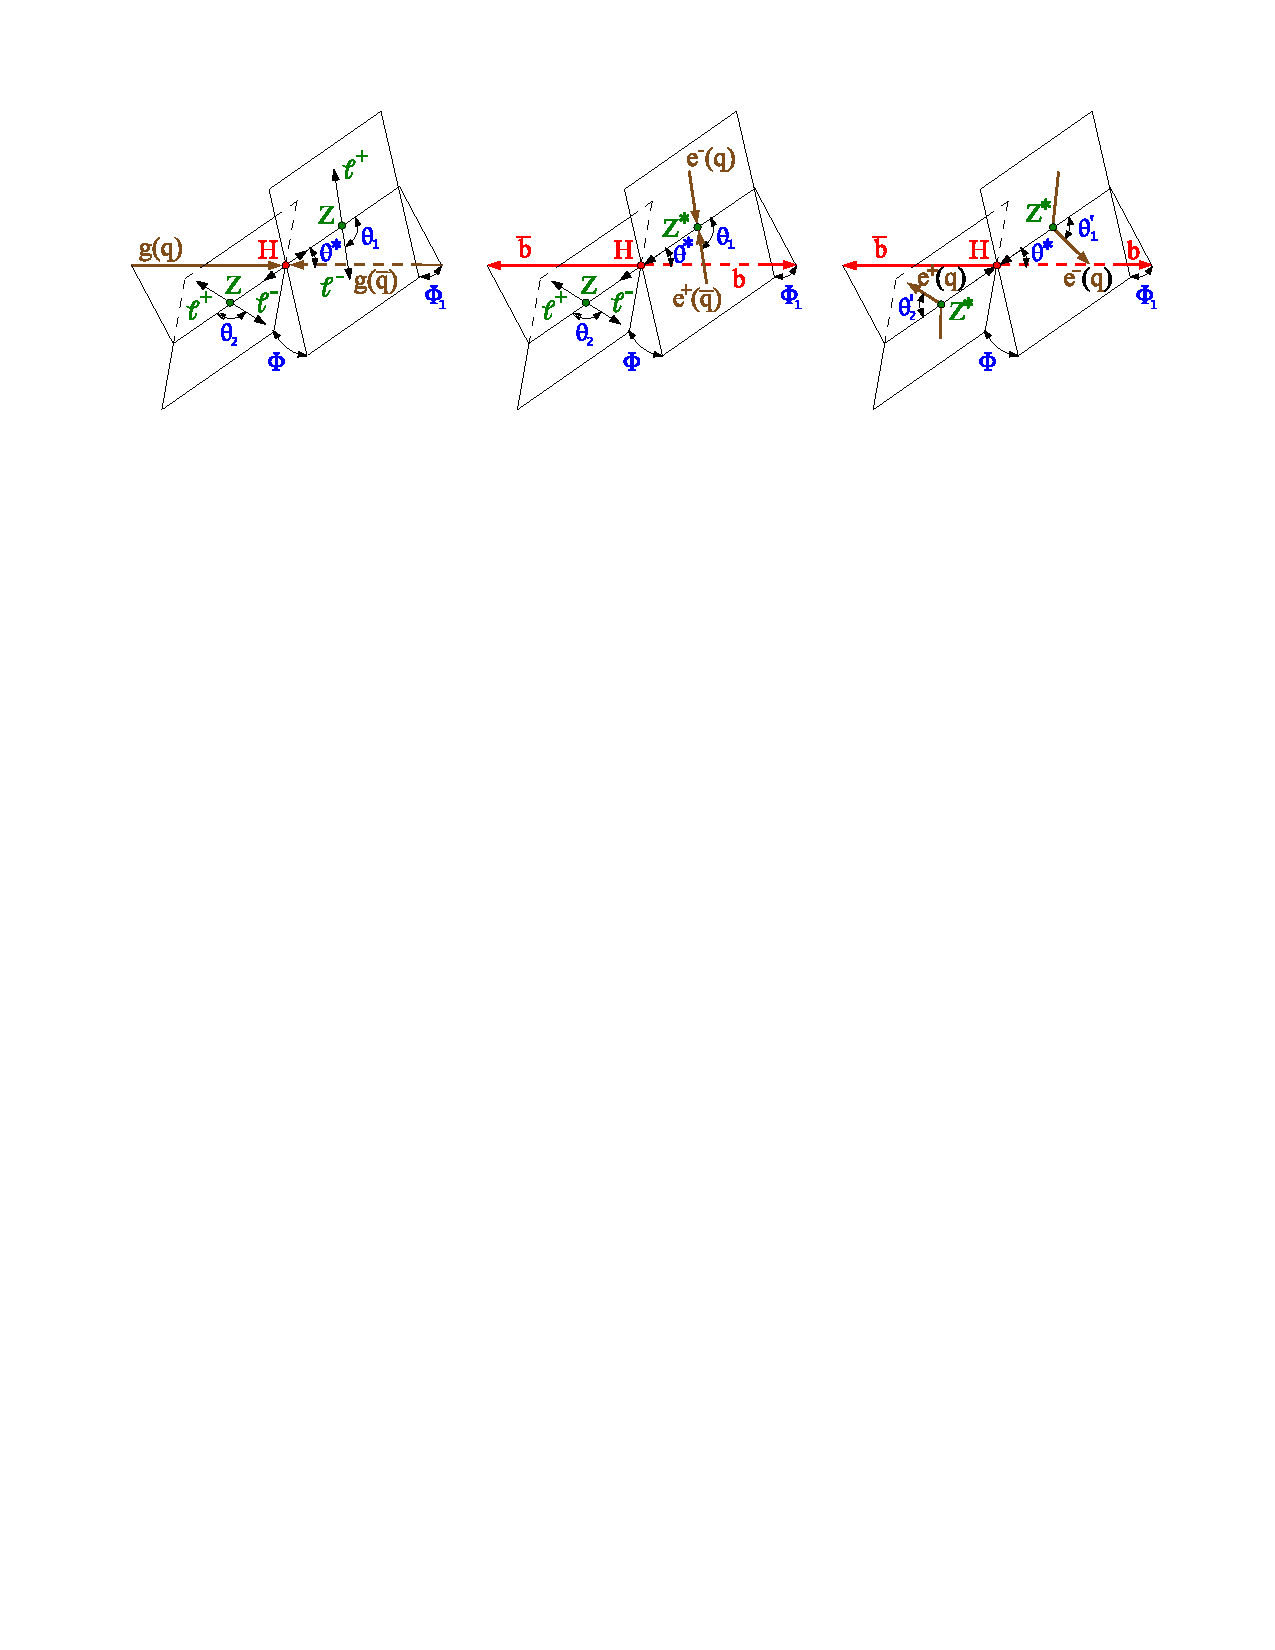
\includegraphics[width=.95\linewidth]{Dissertation/fig/magic-angles.pdf}
\end{center}
\caption{Diagram due to Anderson et. al. \cite{magic-angles-cite} of Higgs-frame angles used for BDT training. The center diagram is most relevant under the following replacements: $Z, Z^*$ to $W, W^*$, $b, \bar{b}$ to $\rho/\phi, \gamma$; $\ell^+,\ell^-$ to $e^-/\mu^-, \nu_e/ \nu_\mu$.}
\label{fig:magic-angles}
\end{figure}

With these features properly defined, we ran the BDT for 200 training rounds with the following model hyperparameters selected to maximize BDT efficiency without overtraining (See Fig. \ref{fig:bdt-knobs} for hyperameter definitions):
\begin{itemize}
    \item \verb|objective| = 'binary:logistic'
    \item \verb|eta| = 0.1
    \item \verb|max_depth| = 3
    \item \verb|verbosity| = 1
    \item \verb|nthread| = 12
    \item \verb|eval_metric| = "auc"
    \item \verb|subsample| = 0.6
    \item \verb|alpha| = 8.0
    \item \verb|gamma| = 2.0
    \item \verb|lambda| = 1.0
    \item \verb|min_child_weight| = 1.0
    \item \verb|colsample_bytree| = 1.0
\end{itemize}

\end{subsection}
\begin{subsection}{Performance and Validation}
We determined satisfactory performance by evaluating the BDT's ROC curves for testing and training (Fig. \ref{fig:bdt-performance}) as well as the sanity of the BDT's feature rankings (Fig. \ref{fig:bdt-vars}). We also checked for background sculpting by two methods. First, we looked at the plot of the BDT scores versus the reconstructed Higgs mass (Fig. \ref{fig:bdt-bkgsculpt1}). A correlation between high BDT scores and the known Higgs mass (125 GeV) would indicate that the BDT was simply learning and cutting on the reconstructed Higgs mass and thus sculpting the background. Second, we directly evaluated the background and signal distributions before and after making a tight cut ($D > 0.9$) on the BDT discriminant, where an artificial peak of the background inside of the signal region would directly show that the BDT was sculpting the background. We required that the BDT pass these two tests before proceeding to use it in the rest of the analysis.

\begin{figure}[htb]
\begin{center}
\begin{tabular}{llll}
\toprule
cut &       gain &       cover &  weight \\
\midrule
$I_{rel}(\phi)$ &  64.823995 &  410.500067 &      57 \\
$\Delta R(K^{+}, K^{-})$ &  49.762952 &  315.353542 &     143 \\
$m_{Z}$ &  34.554528 &  292.716951 &     107 \\
$p_{T}(\phi)$ &  30.415027 &  256.183022 &     123 \\
$m_{\phi}$ &  21.122510 &  374.886933 &      79 \\
$\Delta R(\phi, \gamma)$ &  15.631570 &  256.192849 &     100 \\
$p_{T}(\gamma)$ &  13.298290 &  179.156460 &      46 \\
$\cos\theta_{1}$ &  10.042543 &  346.471954 &      58 \\
$I_{rel}(\gamma)$ &   9.113523 &  269.280112 &      38 \\
$\cos\theta^{*}$ &   7.324339 &  188.648235 &      52 \\
\bottomrule
\end{tabular}

\end{center}
\caption{Top ten variables as ranked by the BDT by gain. All input variables are reconstruction-level Monte Carlo data, and all $p_{T}$ variables are scaled by $m_{H}.$}
\label{fig:bdt-vars}
\end{figure}

\begin{figure}[htb]
\begin{center}
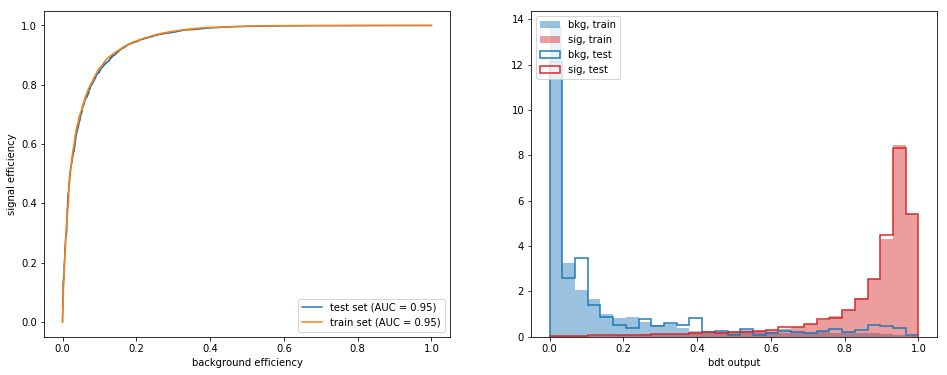
\includegraphics[width=.95\linewidth]{Dissertation/fig/bdt-performance.png}
\end{center}
\caption{Left: ROC curve showing BDT testing (blue) and training (orange) performance. Right: Background (blue) and signal (red) distributions versus BDT score for testing (outline) and training (filled).}
\label{fig:bdt-performance}
\end{figure}

\begin{figure}[htb]
\begin{center}
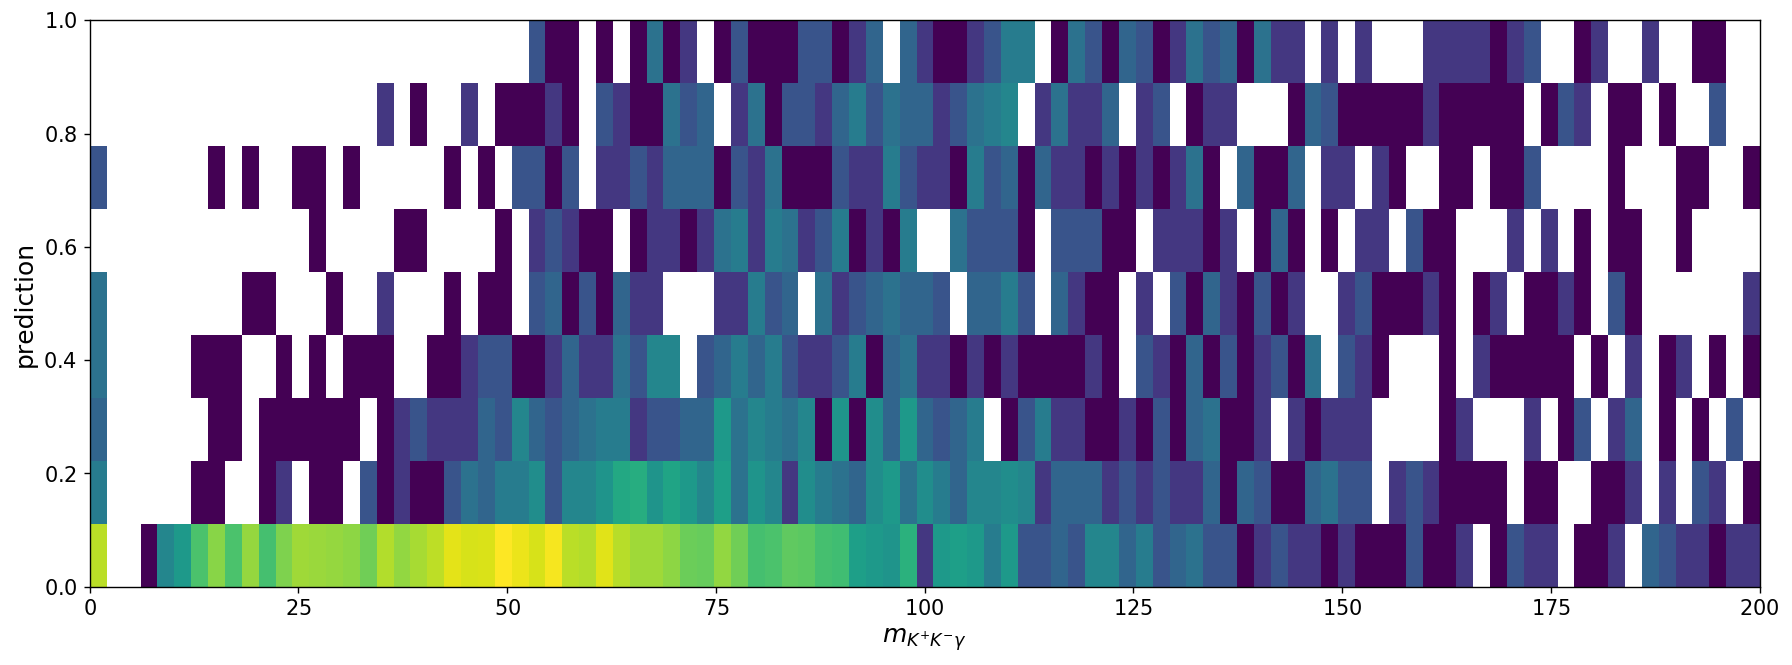
\includegraphics[width=.95\linewidth]{Dissertation/fig/bdt-bkgsculpt1.png}
\end{center}
\caption{Plot of the BDT score versus the reconstructed Higgs mass. A heavy correlation between high score and the true Higgs mass would suggest background is being sculpted.}
\label{fig:bdt-bkgsculpt1}
\end{figure}

\begin{figure}[htb]
\begin{center}
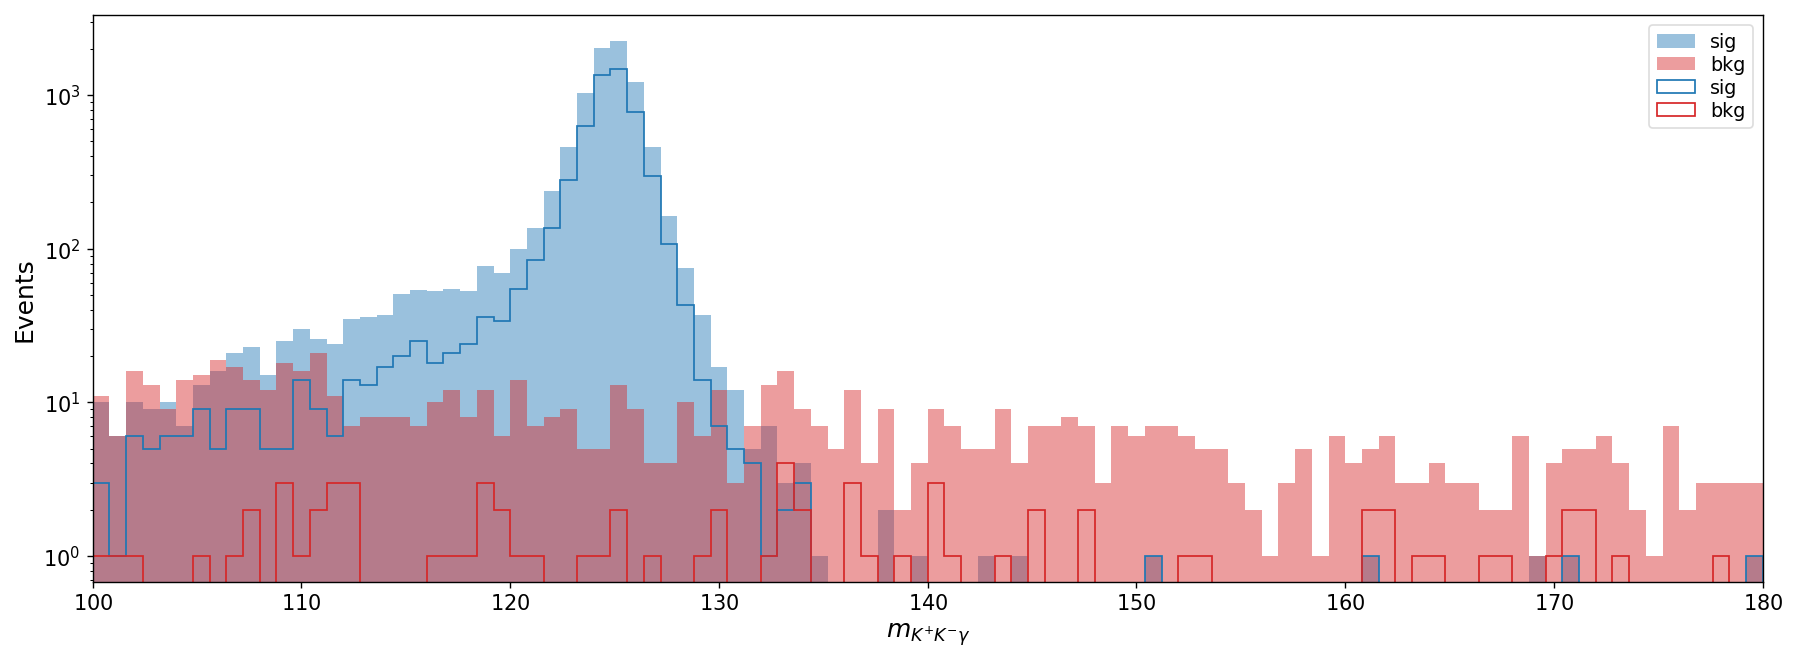
\includegraphics[width=.95\linewidth]{Dissertation/fig/bdt-bkgsculpt2.png}
\end{center}
\caption{Reconstructed Higgs mass distribution for signal (blue) and background (red) before (filled) and after (outline) requiring $D > 0.9$ where $D$ is the BDT discriminant.}
\label{fig:bdt-bkgsculpt2}
\end{figure}
\end{subsection}
\begin{subsection}{Comparison to Cut-Based Approach}
Based on the following basic study, we found that a Boosted Decision Tree (BDT) trained on Monte Carlo simulations of signal and background performed 20\% to 25\% better than traditional, cut-based methods. We determined an optimal BDT working point by sampling the BDT's ROC curve (generated using testing data and predictions) at each defined threshold value, then calculating an expected significance ($\sigma$) defined as:
\begin{equation}\label{expsig-eq}
    \sigma = \sqrt{2(s+b)\ln(1+s/b)-2s}
\end{equation}
\noindent where $s$ and $b$ are the number of signal and background events for a given threshold value. The optimal BDT working point is then given by the maximum $\sigma$-value. Next, we defined a general cut-based approach by the following cuts:
\begin{itemize}
    \item $1.0 < m_{\phi} < 1.04\textnormal{ GeV}$
    \item $\Delta R(K^{+}, K^{-}) < 0.015$
    \item $p_{T}(\phi) > 25\textnormal{ GeV}$
    \item $p_{T}(\gamma) > 40\textnormal{ GeV}$
    \item $I_{rel}(\phi) < 0.01$
\end{itemize}
\noindent Finally, we calculated the false-positive and true-positive rates of the cut-based methods and plotted them against the BDT's ROC curve. The results of this study are plotted in Fig. \ref{fig:bdt-vs-cuts}. Note that the terms BDT ``score," ``threshold," and ``discriminant" will be used interchangeably throughout the remainder of this paper with the understanding that they are the same quantity $D \in [0,1]$.

\begin{figure}[htb]
\begin{center}
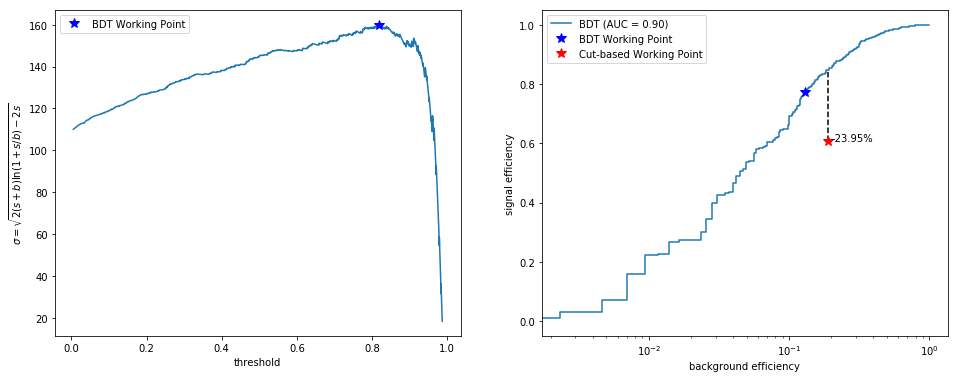
\includegraphics[width=.95\linewidth]{Dissertation/fig/bdt-vs-cuts.png}
\end{center}
\caption{Left: Expected significance ($\sigma$) versus BDT threshold value. Right: Comparison between an optimal BDT working point and cut-based method plotted on top of the BDT's ROC curve.}
\label{fig:bdt-vs-cuts}
\end{figure}
\end{subsection}
\begin{subsection}{Optimization for Data}
With the BDT validated, we proceeded to calculated a proper BDT working point for cutting on data. We noticed that the Monte Carlo samples were not properly modeling the data in the signal region of the BDT discriminant (Fig. \ref{fig:bdt-thresh-dist}). Thus, we concluded that we could not sample the BDT testing ROC curve for an effective working point. Instead, we fed the BDT ROC curve data as background in addition to signal Monte Carlo. We then sampled this distribution, calculated expected significance again using Eq. \ref{expsig-eq}, and took the best BDT working point to be at the threshold with maximum expected significance (Fig. \ref{fig:bdt-data-expsig}).

\begin{figure}[htb]
\begin{center}
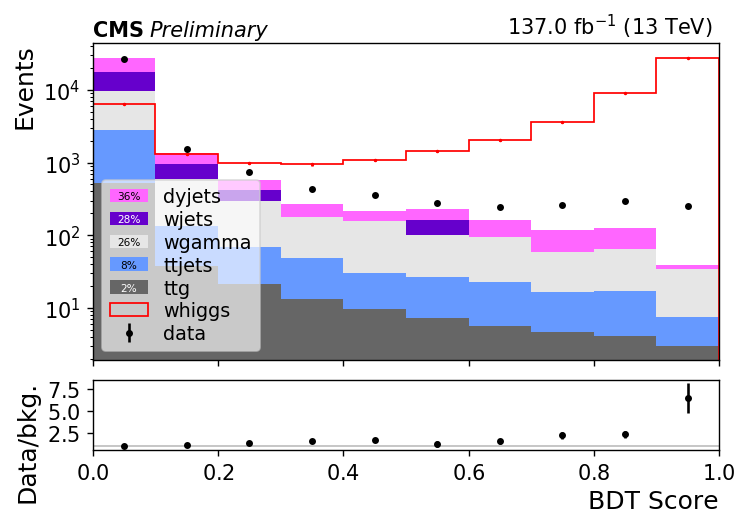
\includegraphics[width=.95\linewidth]{Dissertation/fig/bdt-threshBySample.png}
\end{center}
\caption{Stacked BDT discriminant distribution plot by sample.}
\label{fig:bdt-thresh-dist}
\end{figure}

\begin{figure}[htb]
\begin{center}
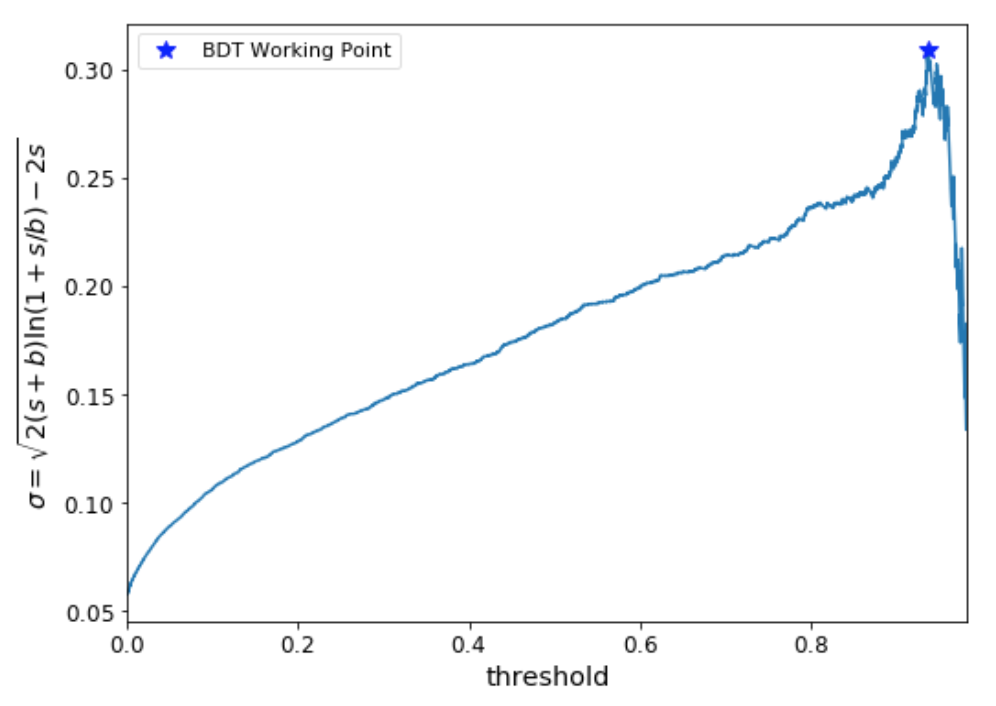
\includegraphics[width=.95\linewidth]{Dissertation/fig/bdt-data-expsig.png}
\end{center}
\caption{Expected significance versus BDT threshold.}
\label{fig:bdt-data-expsig}
\end{figure}

\end{subsection}
\end{section}

\begin{section}{Results}
Lorem ipsum dolor sit amet, consectetur adipiscing elit. Quisque eu eros nisl. Donec sollicitudin nisl nisi, sit amet rutrum nibh faucibus sit amet. In a efficitur dui. Nunc at sagittis urna. Quisque venenatis nec risus quis eleifend. Fusce id nulla in urna tristique iaculis. In et consectetur risus, nec commodo justo. In augue enim, efficitur ac commodo quis, tempus ac arcu. Sed porta dolor ultrices, pellentesque tellus eu, mollis mi. Phasellus et condimentum odio. Curabitur condimentum rhoncus sem, eget sagittis eros rhoncus sit amet. Class aptent taciti sociosqu ad litora torquent per conubia nostra, per inceptos himenaeos. Maecenas ac felis aliquam orci eleifend faucibus vitae sit amet mauris. Fusce vel magna mi. Aenean commodo pellentesque tellus, ut iaculis est auctor et.
Aliquam porttitor justo dolor. Duis ut ex lacinia, vulputate dui a, molestie lorem. Vestibulum elementum lectus vel mollis iaculis. Cras ante purus, pellentesque sit amet sem sed, convallis dapibus est. Aenean vehicula mollis bibendum. Integer aliquet condimentum luctus. Suspendisse vitae rhoncus justo.
\end{section}

\begin{figure}[htb]
\begin{center}
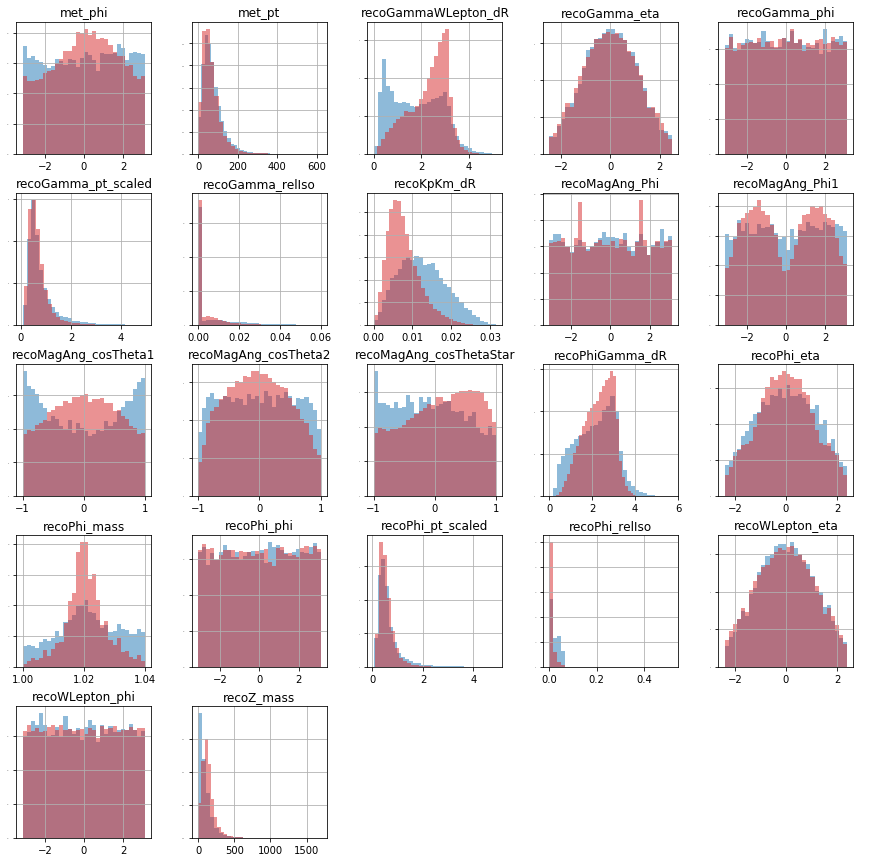
\includegraphics[width=.95\linewidth]{Dissertation/fig/bdt-training.png}
\end{center}
\caption{Preliminary histograms for every feature used to train the BDT. These were drawn before any weights are applied, so they do not completely represent what the BDT saw, however they do provide some insight into the motivation behind the BDT's variable rankings.}
\label{fig:bdt-training}
\end{figure}

\appendix

\dsp

\chapter{Technical Details}
\begin{section}{CMS Coordinate System}

In the CMS Coordinate system, the $z$-axis is aligned along the beampipe, therefore running parallel to the barrel and perpendicular to the endcap of the detector. The $x$-axis points radially towards the center of the LHC, and the y-axis points orthogonal to $x$ and $z$. The azimuthal angle $\phi$ is defined about the $z$-axis, as in cylindrical coordinates, and the pseudo-rapidity $\eta$ is defined as

\begin{equation}
    \eta \equiv -\ln{\bigg[ \tan{\bigg( \frac{\theta}{2} \bigg)} \bigg]}
\end{equation}

\noindent where $\theta$ is the angle between the particle three-momentum and positive $z$-axis. See Figure \ref{fig:cms-coords} for a visualization of this coordinate system.

\begin{figure}[htb]
\begin{center}
\tdplotsetmaincoords{75}{50} % to reset previous setting
\begin{tikzpicture}[scale=2.7,tdplot_main_coords,rotate around x=90]
 
  % variables
  \def\rvec{1.2}
  \def\thetavec{40}
  \def\phivec{70}
  \def\R{1.1}
  \def\w{0.3}
 
  % axes
  \coordinate (O) at (0,0,0);
  \draw[thick,->] (0,0,0) -- (1,0,0) node[below left]{$x$};
  \draw[thick,->] (0,0,0) -- (0,1,0) node[below right]{$y$};
  \draw[thick,->] (0,0,0) -- (0,0,1) node[below right]{$z$};
  \tdplotsetcoord{P}{\rvec}{\thetavec}{\phivec}
 
  % vectors
  \draw[->,red] (O) -- (P) node[above left] {$P$};
  \draw[dashed,red] (O)  -- (Pxy);
  \draw[dashed,red] (P)  -- (Pxy);
  \draw[dashed,red] (Py) -- (Pxy);
 
  % circle - LHC
  \tdplotdrawarc[thick,rotate around x=90,black!70!blue]{(\R,0,0)}{\R}{0}{360}{}{}
 
  % compass - the line between CMS and ATLAS has a ~12° declination (http://googlecompass.com)
  \begin{scope}[shift={(1.1*\R,0,1.65*\R)},rotate around y=12]
    \draw[<->,black!50] (-\w,0,0) -- (\w,0,0);
    \draw[<->,black!50] (0,0,-\w) -- (0,0,\w);
    \node[above left,black!50,scale=0.6] at (-\w,0,0) {N};
  \end{scope}
 
  % nodes
  \node[left,align=center] at (0,0,1.1) {Jura};
  \node[right] at (\R,0,0) {LHC};
  \fill[radius=0.8pt,black!20!red]
    (O) circle node[left=4pt,below=2pt] {CMS};
  \draw[thick] (0.02,0,0) -- (0.5,0,0); % partially overdraw x-axis and CMS point
  \fill[radius=0.8pt,black!20!blue]
    (2*\R,0,0) circle
    node[right=4pt,below=2pt,scale=0.9] {ATLAS};
  \fill[radius=0.8pt,black!10!orange]
    ({\R*sqrt(2)/2+\R},0,{ \R*sqrt(2)/2}) circle % 45 degrees from ATLAS
    node[left=2pt,below=2pt,scale=0.8] {ALICE};
  \fill[radius=0.8pt,black!60!green]
    ({\R*sqrt(2)/2+\R},0,{-\R*sqrt(2)/2}) circle % 45 degrees from ATLAS
    node[below=2pt,right=2pt,scale=0.8] {LHCb};
 
  % arcs
  \tdplotdrawarc[->]{(O)}{0.2}{0}{\phivec}
    {above=2pt,right=-1pt,anchor=mid west}{$\varphi$}
  \tdplotdrawarc[->,rotate around z=\phivec-90,rotate around y=-90]{(0,0,0)}{0.5}{0}{\thetavec}
    {anchor=mid east}{$\eta$}
 
\end{tikzpicture}
\end{center}
\caption{Diagram of CMS coordinate system.}
\label{fig:cms-coords}
\end{figure}

\end{section}

\begin{section}{Boosted Decision Trees}
A Boosted Decision Tree (BDT) is simply an extension of a decision tree, which is can be visualized as follows: starting from a single ``node," two ``branches" emerge; at the end of each branch, there is another node that also joins two branches, and so on. In this picture, each node is a binary decision (i.e. $A > B$, $C == D$, etc.) and the two branches joined by each node represent the path ``traveled" by data should it pass or fail -- hence \textit{two} branches -- the condition. The tree may be optimized by recursively adding nodes and adjusting the ``splits" (the exact value over which the input is split) at each node until some given condition is met such that an optimal configuration is reached. This is essentially an accurate representation of the classical, ``cut-based" analysis that has been performed in High Energy for decades, where physicists filter out everything they are not looking for (background) with the hope that what they are looking for (signal) remains after the surrounding noise is cleared. A similar (both in practice is results) optimization of this technique is achieved by a combination of educated insight and trail and error. Thus, it is clear that the computational method of the decision tree would fit into the workflow of a High Energy physics analysis, but a decision tree is not an exceptionally powerful classifier on its own. However, they can be ``boosted" by creating several decision trees, collecting their output, and calculating a value called a ``determinant" (henceforth referred to as $D$), forming a stronger classifier from the collection of weak ones. The exact process of constructing and optimizing a BDT is dependent on the particular algorithm used and is beyond the scope of this paper. For the interested reader, more information on XGBoost, the algorithm used for this paper, can be found here\cite{cite-xgboost}.
\end{section}

\end{mainmatter}

%----- Bibliography ----------------
\ssp
\bibliographystyle{JHEP3}
\bibliography{dissertation}

\end{document} 
